% !TEX program = xelatex
% !TEX TS-program = xelatex
% !TEX encoding = UTF-8 Unicode

\documentclass[a4paper, 12pt]{article}
\usepackage{amsmath}
\usepackage{fontspec}  % 解决中文问题
	\defaultfontfeatures{Mapping=tex-text}
	\setromanfont{Songti SC}  % Mac下使用此句
	% \setromanfont{"[msyh.ttc]"}  % Windows下使用此句
	\XeTeXlinebreaklocale “zh”
	\XeTeXlinebreakskip = 0pt plus 1pt minus 0.1pt
\usepackage[top=20mm, bottom=25mm, left=20mm, right=25mm]{geometry}  % 设置页边距
	% \special{papersize=12cm,9cm}  % For Kindle
	% \setlength\paperheight{35cm}  % For iPhone 7
	% \setlength\paperwidth{20cm}
\usepackage{tikz}  % 画图用s
	\def\pgfsysdriver{pgfsys-dvipdfmx.def}
\usepackage{xltxtra}
\usepackage{xunicode}

\renewcommand{\thefootnote}{注[\arabic{footnote}]}  % 重新定义\footnote命令的格式


\usepackage[colorlinks,linkcolor=blue]{hyperref}  % 设置超链接

\graphicspath{{../}}



\begin{document}
	\title{机器学习笔记}
\author{MingShun Wu}
\date{\today}
\maketitle
	\renewcommand{\contentsname}{目录}
\tableofcontents
\setcounter{tocdepth}{3}
	
	\section*{说明}
\begin{enumerate}
	\item 本文是根据吴恩达(Andrew Ng) CS229课程的视频\&讲义,再加上一些自己的理解整理出来的,我也只是个初学者,里面的内容可能有很多错误,若发现错误欢迎联系我修改: \href{mailto:wu.mingshun@icloud.com}{wu.mingshun@icloud.com}
	\item 暂时只有部分内容,通过后面的网址可以下载到最新的文档(若有更新会替换掉原来的文件),下载最新文档:\href{http://images.miasun.cn/math/CS299课程笔记.pdf}{http://images.miasun.cn/math/CS299课程笔记.pdf}
	% \item 
	% 个人联系方式:
	% \begin{enumerate}
	% 	\item 邮件:
	% 	\item 微信
	% 	\begin{figure}[htbp]
	% 		\centering
	% 		
\includegraphics[scale=0.25]{images/微信号二维码}
	% 		\caption{微信号二维码}
	% 	\end{figure}
	% \end{enumerate}
	
\end{enumerate}






























	\section{线性回归}
\subsection{假设函数(Hypothesis Function)}
\begin{equation}\begin{aligned}
	h_\theta(x) = \theta_0 + \theta_1x_1 + \theta_2x_2 + \theta_3x_3 + ... + \theta_nx_n
\end{aligned}\end{equation}
另$x_0=1$,则
\begin{equation}\begin{aligned}
	h_\theta(x) &= \theta_0x_0 + \theta_1x_1 + \theta_2x_2 + \theta_3x_3 + ... + \theta_nx_n \\
	&= \sum_{j=0}^n{\theta_jx_j}
\end{aligned}\end{equation}

\subsection{最小二乘法}
梯度下降中的Cost Function均使用的时最小二乘法

\subsection{梯度下降}
\subsubsection{批梯度下降(BGD)}
\begin{enumerate}
	\item Cost Function
	\begin{equation}\begin{aligned}
		J(\theta) = \frac{1}{2} \sum_{i=1}^m \left[h_{\theta} {(x^{(i)})} - y^{(i)}\right]^2
	\end{aligned}\end{equation}
	其中,$J(\theta)$就是在训练过程中的Cost Function。我们的目的就是将该Cost Function最小化。
	在以上式子中:\\
		$x^{(i)}$为训练集的输入;\\
		$y^{(i)}$为训练集的输出;\\
		$\theta$为所要训练的参数;\\
		$h_{\theta}$为假设函数;\\
		$h_{\theta} {(x^{(i)})}$为训练集输入经过假设函数后得到的结果\\
		以上式子中,其实是使用最小二乘法

	\item 迭代方式
	\begin{equation}\begin{aligned}
	      \theta_j &:= \theta_j - \alpha \frac{\partial} {\partial \theta_j} J(\theta)
	\end{aligned}\end{equation}
	其中:
	\begin{equation}\begin{aligned}
	      \frac{\partial} {\partial \theta_j} J(\theta) &= \frac{\partial}{\partial \theta_j} \frac{1}{2} \sum_{i=1}^m\left[ h_\theta(x^{(i)}) - y^{(i)} \right]^2 \\
	      &= 2 * \frac{1}{2} \sum_{i=1}^m\left[ h_\theta(x^{(i)}) - y^{(i)} \right] \frac{\partial}{\partial\theta_j}\left[ h_\theta(x^{(i)}) - y^{(i)} \right] \\
	      &= \sum_{i=1}^m\left[ h_\theta(x^{(i)}) - y^{(i)} \right]\frac{\partial}{\partial\theta_j}\left[ \theta_0x_0^{(i)} +  \theta_1x_1^{(i)} + \theta_2x_2^{(i)} + ... + \theta_nx_n^{(i)} - y^{(i)} \right] \\
	      &= \sum_{i=1}^m\left[ h_\theta(x^{(i)}) - y^{(i)} \right]x_j^{(i)}
	\end{aligned}\end{equation}
	所以,更新后的梯度下降公式为
	\begin{equation}\begin{aligned}
		\theta_j &:= \theta_j - \alpha \sum_{i=1}^m \left[ h_\theta(x^{(i)}) - y^{(i)} \right]x_j^{(i)}
	\end{aligned}\end{equation}
	其中,$\alpha$称为学习速率(learning rate),用于控制$\theta$前进的步伐,避免$\theta$走得太快(或太慢)。\\

	梯度下降法每次计算都是找到当前所在位置中,下降最快的方向(至于为什么是当前所在位置中下降最快的方向就是梯度的定义了)。 \\
	如果计算进入了某个局部极小值,则很可能一直在这个局部极小值内出不来了(除非你的步长比较大,帮助它跑出这个局部极小值),这就是梯度下降法的局限所在,它很容易陷入局部极小值中。 \\
	使用梯度下降法每次修正的时参数$\theta$,而不是输入的$X$或$y$ \\

	Todo PS: 以下内容正确性待思考。因为其是当前位置下,下降最快的方向,若出现每个维度求导后结果都是0,则此时不论再怎么迭代,这个点都不会再变化了(或者其他导致每个维度的偏导数都为0的情况也类似,当然,这种情况较少见)
\end{enumerate}


\subsubsection{随机梯度下降(SGD)}
由批梯度下降的式子可以发现,在每一次梯度下降的迭代过程中,我们遍历了所有训练集。这将会耗费大量的性能,于是产生了随机梯度下降(SGD)方法,每次迭代只使用一个数据。 \\
\begin{enumerate}
	\item Cost Function
	\begin{equation}\begin{aligned}
		J(\theta) = \frac{1}{2} \left[h_{\theta} {(x^{(i)})} - y^{(i)}\right]^2
	\end{aligned}\end{equation}

	\item 迭代方式
	\begin{equation}\begin{aligned}
	      \frac{\partial} {\partial \theta_j} J(\theta) &= \left[ h_\theta(x^{(i)}) - y^{(i)} \right]x_j^{(i)}
	\end{aligned}\end{equation}
	更新后的梯度下降公式为
	\begin{equation}\begin{aligned}
		\theta_j &:= \theta_j - \alpha\left[ h_\theta(x^{(i)}) - y^{(i)} \right]x_j^{(i)}
	\end{aligned}\end{equation}
	如上所示,与批梯度下降不同,随机梯度下降每次迭代只用了一个数据(第$i$个数据),若$i$从1取到m,则完成了一次训练集的遍历。\\
	使用随机梯度下降虽然解决了批梯度下降耗费过多性能的问题,但是却带来了另一个问题:收敛太慢!由此,我们折中使用迷你批梯度下降(mini-batch GD)。\\
	随机梯度下降(包括其他梯度下降方法)均允许多次遍历所有数据集。
\end{enumerate}

\subsubsection{迷你批梯度下降(mini-batch GD)}
为了解决梯度下降每次都使用所有训练集导致的性能问题,以及随机梯度下降每次只使用一个数据导致的收敛太慢,我们可以只用mini-batch GD。每次只用一部分训练集进行训练。
\begin{enumerate}
	\item Cost Function \\
	略

	\item 迭代方式 \\
	略
\end{enumerate}











		\subsection{线性代数知识}
\begin{enumerate}
	\item
	\begin{equation}
		\nabla_{\theta}J(\theta) = \left[\begin{matrix}
		\frac{\partial J}{\partial\theta_0} \\
		\frac{\partial J}{\partial\theta_1} \\
		\vdots \\
		\frac{\partial J}{\partial\theta_n} \\
		\end{matrix}\right], \quad \in {\rm I\!R}^{n+1}
	\end{equation}

	\item
	\begin{equation}
		\nabla_Af(A) = \left[ \begin{matrix}
			\frac{\partial f}{\partial A_{11}} & \frac{\partial f}{\partial A_{12}} & \dots & \frac{\partial f}{\partial A_{1n}} \\
			\frac{\partial f}{\partial A_{21}} & \frac{\partial f}{\partial A_{22}} & \dots & \frac{\partial f}{\partial A_{2n}} \\
			\vdots & \vdots & \ddots & \vdots \\
			\frac{\partial f}{\partial A_{n1}} & \frac{\partial f}{\partial A_{n2}}& \dots & \frac{\partial f}{\partial A_{nn}} \\
		\end{matrix}\right]
	\end{equation}

	\item 矩阵的迹的计算方式 \\
	如果矩阵$A$是方阵,则:
	\begin{equation}
		tr(A) = \sum_{i=1}^nA_{ii}
	\end{equation}

	\item 矩阵的迹的性质
	\begin{equation}
		tr(AB) = tr(BA)
	\end{equation}
	\begin{equation}
		tr(ABC) = tr(CAB) = tr(BCA)
	\end{equation}
	\begin{equation}
		tr(A^T) = tr(A)
	\end{equation}
	\begin{equation}
		tr(A+B) = trA + trB
	\end{equation}
	\begin{equation}
		traA = atrA
	\end{equation}

	\item 
	\begin{equation}
		\nabla_AtrAB = B^T
	\end{equation}
	\begin{equation}
		\nabla_{A^T}f(A) = (\nabla_Af(A))^T
	\end{equation}
	\begin{equation}
		\nabla_AtrABA^TC = CAB + C^TAB^T
	\end{equation}
	\begin{equation}
		\nabla_A|A| = |A|(A^{-1})^T
	\end{equation}
	\begin{equation}
		A^{-1} = \frac{(A^{'})^T}{|A|}
	\end{equation}
	其中,$A^{-1}$为矩阵的逆



\end{enumerate}



















		\subsection{梯度下降过程的矩阵表达}
\begin{enumerate}
	\item 
	\begin{equation}
		X = \left[\begin{matrix}
		-\!-  & (x^{(1)})^T & -\!- \\
		-\!- & (x^{(2)})^T & -\!- \\
		\vdots & \ddots & \vdots \\
		-\!- & (x^{(m)})^T & -\!- \\
		\end{matrix}\right] \quad \in {\rm I\!R}^{m \times (n+1)}
	\end{equation}

	\item 
	\begin{equation}
		\vec{y} = \left[\begin{matrix}
		y^{(1)} \\ y^{(2)} \\ \vdots \\ y^{(m)}
		\end{matrix}\right] \quad \in {\rm I\!R}^{m \times 1}
	\end{equation}

	\item 
	\begin{equation}
		X\theta - \vec{y} = \left[\begin{matrix}
		(x^{(1)})^T\theta \\ (x^{(2)})^T\theta \\ \vdots \\ (x^{(m)})^T\theta
		\end{matrix}\right] - \left[\begin{matrix}
		y^{(1)} \\ y^{(2)} \\ \vdots \\ y^{(m)}
		\end{matrix}\right] = \left[\begin{matrix}
		h_\theta(x^{(1)}) - y^{(1)} \\ h_\theta(x^{(2)}) - y^{(2)} \\ \vdots \\ h_\theta(x^{(m)}) - y^{(m)}
		\end{matrix}\right]  \quad \in {\rm I\!R}^{m \times 1}
	\end{equation}

	\item 
	\begin{equation}
		J(\theta) = \frac{1}{2}(X\theta - \vec{y})^T(X\theta - \vec{y})
	\end{equation}
	\footnote{这就是矩阵中平方的表达方式}

	\item 
	\begin{equation}
		\nabla_{\theta}J(\theta) = X^TX\theta - X^T \vec{y}
	\end{equation}
	为了得到最值,另上式值为0(极值点的方向倒数均为0),可得
	\begin{equation}
		\theta = (X^TX)^{-1}X^T\vec{y}
	\end{equation}






\end{enumerate}




























		\subsection{线性回归中使用最小二乘法的合理性解释}
\subsubsection{证明过程}
\begin{enumerate}
	\item 我们可以将实际的$y^{(i)}$分为两个部分:一部分被我们的计算模型所包括,为$\theta^Tx^{(i)}$;一部分未被我们的计算模型所包括,将其记为$\epsilon^{(i)}$,可得:
	\begin{equation}
		y^{(i)} = \theta^Tx^{(i)} + \epsilon^{(i)}
	\end{equation}

	\item 根据中心极限定理\footnote{中心极限定理大意:许多独立随机变量之和趋向于服从高斯分布。 更详细的待补充...},同时根据经验,我们可以假设$\epsilon^{(i)}$服从高斯分布$N(\mu, \sigma^2)$,故
	\begin{align}
		p(\epsilon^{(i)}) &= \frac{1}{\sqrt{2\pi}\sigma}e^{-\frac{\left(\epsilon^{(i)}-\mu\right)^2}{2\sigma^2}}  \\
		&\downarrow \\
		p(y^{(i)}|x^{(i)};\theta) &= \frac{1}{\sqrt{2\pi}\sigma}e^{-\frac{\left(y^{(i)}-\theta^Tx^{(i)}-\mu\right)^2}{2\sigma^2}}
	\end{align}
	\footnote{在数学上,对于连续型随机变量,$F(x)$表示随机变量的分布函数,$f(x)$表示其概率密度,二者表示的数学意义不一样,且$F'(x) = f(x)$;对于离散型来讲$P(X=x_i)=p_i$,两个值意义一样且都叫分布律}

	\item 写出其似然函数
	\begin{align}
		L(\theta) &= L(\theta; X, \vec{y}) = p(\vec{y}|X; \theta) \\
		&= \prod_{i=1}^{m}P(y^{(i)}|x^{(i)}; \theta) \\
		&= \prod_{i=1}^{m}\frac{1}{\sqrt{2\pi}\sigma}e^{-\frac{\left(y^{(i)}-\theta^Tx^{(i)}-\mu\right)^2}{2\sigma^2}} \\
		&= \left(\frac{1}{\sqrt{2\pi}\sigma}\right)^m\cdot e^{\sum_{i=1}^{m}{-\frac{\left(y^{(i)}-\theta^Tx^{(i)}-\mu\right)^2}{2\sigma^2}}}
	\end{align}
	\footnote{关于此式子的理解建议看看文档末尾附录中对似然函数的介绍。}

	\item 显然,求其对数后更好分析
	\begin{align}
		l(\theta) &= \ln{L(\theta)} \\
		&= \ln\left[\left(\frac{1}{\sqrt{2\pi}\sigma}\right)^m\cdot e^{\sum_{i=1}^{m}{-\frac{\left(y^{(i)}-\theta^Tx^{(i)}-\mu\right)^2}{2\sigma^2}}}\right] \\
		&= m\cdot\ln\frac{1}{\sqrt{2\pi}\sigma} - \sum_{i=1}^{m}\frac{\left(y^{(i)}-\theta^Tx^{(i)}-\mu\right)^2}{2\sigma^2} \\
		&= m\cdot\ln\frac{1}{\sqrt{2\pi}\sigma} - \frac{1}{{\sigma^2}}\cdot \frac{1}{2} \sum_{i=1}^{m}\left(y^{(i)}-\theta^Tx^{(i)}-\mu\right)^2
	\end{align}

	\item 由上式可知,若要最小化似然函数$l(\theta)$,等价于最小化$\frac{1}{2} \sum_{i=1}^{m}\left(y^{(i)}-\theta^Tx^{(i)}-\mu\right)^2$,此式子同样是最小二乘法的形式。令常数项$\mu = 0$便可得到前述线性回归Cost Function使用的最小二乘法,故在线性回归中使用最小二乘法计算$J(\theta)$是合理的

\end{enumerate}

\subsubsection{说明}
\begin{enumerate}
	\item 从上述结果中,我们可以发现,让$l(\theta)$取到最值时的$\theta$值与$\sigma^2$无关。后续说明指数分布族\&广义线性模型时将会用到此性质
\end{enumerate}














		\subsection{线性回归的代码实现}

\subsubsection{各向量形式}
在机器学习中,各个变量在单独出现时均为列向量的形式,但若是以多个向量形成的矩阵形式出现时,均为行向量的形式。\\
以下将会写出各个变量单独出现的情况、各变量以矩阵的形式一起出现的情况。
\begin{enumerate}
\item $\vec{x}$
\begin{equation}
	\vec{x} = \left(\begin{matrix}
				x_0 \\ x_1 \\ x_2 \\ \vdots \\ x_n
			\end{matrix}\right)
			= \left(\begin{matrix}
				1 \\ x_1 \\ x_2 \\ \vdots \\ x_n
			\end{matrix}\right), \quad {\rm I\!R}^{{(n+1)*1}}
\end{equation}

\item $\vec{\theta}$
\begin{equation}
	\vec{\theta} = \left(\begin{matrix}
					\theta_0 \\ \theta_1 \\ \vdots \\ \theta_n
				\end{matrix}\right), \quad {\rm I\!R}^{{(n+1)*1}}
\end{equation}

\item $\vec{y}$
\begin{equation}
	\vec{y} = \left(\begin{matrix}
				y
			\end{matrix}\right), \quad {\rm I\!R}^{1*1}
\end{equation}

% \item $h_{\vec{\theta}}(\vec{x})$
% \begin{equation}\begin{aligned}
% 	h_{\vec{\theta}}(\vec{x}) & = \vec{\theta}^{T}\vec{X} = \vec{X}^T\vec{\theta} \\
% 		& = \left( \begin{matrix}
% 			1 & x_1 & x_2 & \dots & x_n
% 			\end{matrix}\right)
% 			\left(\begin{matrix}
% 				\theta_0 \\
% 				\theta_1 \\
% 				\dots \\
% 				\theta_n
% 			\end{matrix}\right) \\
% 		& = \theta_0 + \theta_1x_1 + \theta_2x_2 + \dots + \theta_nx_n
% \end{aligned} \end{equation}
\end{enumerate}

\subsubsection{批梯度下降}

下述式子中均为矩阵的形式 \\
\begin{enumerate}
\item $X$
\begin{equation} \begin{aligned}
	X & = \left(\begin{matrix}
			\vec{x}^{(1)} \\ \vec{x}^{(2)} \\ \vec{x}^{(3)} \\ \vdots \\ \vec{x}^{(m)}
		\end{matrix}\right) \\
	& = \left( \begin{matrix}
			x_0^{(1)} & x_1^{(1)} & x_2^{(1)} & x_3^{(1)} & \dots & x_n^{(1)} \\
			x_0^{(2)} & x_1^{(2)} & x_2^{(2)} & x_3^{(2)} & \dots & x_n^{(2)} \\
			x_0^{(3)} & x_1^{(3)} & x_2^{(3)} & x_3^{(3)} & \dots & x_n^{(3)} \\
			\vdots    & \vdots    & \vdots    & \vdots    & \ddots & \vdots   \\
			x_0^{(m)} & x_1^{(m)} & x_2^{(m)} & x_3^{(m)} & \dots & x_n^{(m)} \\
			\end{matrix}\right) \\
	& = \left(\begin{matrix}
			1 & x_1^{(1)} & x_2^{(1)} & x_3^{(1)} & \dots & x_n^{(1)} \\
			1 & x_1^{(2)} & x_2^{(2)} & x_3^{(2)} & \dots & x_n^{(2)} \\
			1 & x_1^{(3)} & x_2^{(3)} & x_3^{(3)} & \dots & x_n^{(3)} \\
			\vdots    & \vdots    & \vdots    & \vdots    & \ddots & \vdots   \\
			1 & x_1^{(m)} & x_2^{(m)} & x_3^{(m)} & \dots & x_n^{(m)} \\
		\end{matrix}\right), \quad {\rm I\!R}^{{m*(n+1)}}
\end{aligned} \end{equation}

\item $\vec{\theta}$
\begin{equation} \begin{aligned}
	\vec{\theta} & = \left(\begin{matrix}
			\theta_0 \\ \theta_1 \\ \theta_2 \\ \theta_3 \\ \vdots \\ \theta_n \\
		\end{matrix}\right), \quad {\rm I\!R}^{{(n+1)*1}}
\end{aligned}\end{equation}

\item $h_{\vec{\theta}}(\vec{x})$
\begin{equation}\begin{aligned}
	h_{\vec{\theta}}(\vec{x}) &= X * \vec{\theta} \\
	    & = \left(\begin{matrix}
			1 & x_1^{(1)} & x_2^{(1)} & x_3^{(1)} & \dots & x_n^{(1)} \\
			1 & x_1^{(2)} & x_2^{(2)} & x_3^{(2)} & \dots & x_n^{(2)} \\
			1 & x_1^{(3)} & x_2^{(3)} & x_3^{(3)} & \dots & x_n^{(3)} \\
			\vdots    & \vdots    & \vdots    & \vdots    & \ddots & \vdots   \\
			1 & x_1^{(m)} & x_2^{(m)} & x_3^{(m)} & \dots & x_n^{(m)} \\
		\end{matrix}\right)
		\left(\begin{matrix}
			\theta_0 \\ \theta_1 \\ \theta_2 \\ \theta_3 \\ \vdots \\ \theta_n \\
		\end{matrix}\right) \\
		& = \left(\begin{matrix}
			1\theta_0 + x_1^{(1)}\theta_1 + x_2^{(1)}\theta_2 + x_3^{(1)}\theta_3 + \dots + x_n^{(1)}\theta_n \\
			1\theta_0 + x_1^{(2)}\theta_1 + x_2^{(2)}\theta_2 + x_3^{(2)}\theta_3 + \dots + x_n^{(2)}\theta_n \\
			1\theta_0 + x_1^{(3)}\theta_1 + x_2^{(3)}\theta_2 + x_3^{(3)}\theta_3 + \dots + x_n^{(3)}\theta_n \\
			\vdots \\
			1\theta_0 + x_1^{(m)}\theta_1 + x_2^{(m)}\theta_2 + x_3^{(m)}\theta_3 + \dots + x_n^{(m)}\theta_n \\
		\end{matrix}\right), \quad {\rm I\!R}^{{m*1}}
\end{aligned}\end{equation}

\item $\vec{y}$
\begin{equation}
	\vec{y} = \left(\begin{matrix}
		y^{(1)} \\ y^{(2)} \\ y^{(3)} \\ \vdots \\ y^{(m)}
	\end{matrix}\right), \quad {\rm I\!R}^{{m*1}}
\end{equation}
\end{enumerate}

\subsubsection{Cost Function}
\begin{enumerate}
\item 数值计算形式:
\begin{equation}
	J(\theta) = \frac{1}{2m} \sum_{i=1}^m \left[ h_\theta(x^{(i)}) - y^{(i)}\right]^2
\end{equation}

\item 矩阵计算形式:
\begin{equation}
	J(\theta) = \frac{1}{2m} \left[h_{\vec{\theta}}(\vec{x}) - \vec{y}\right]^T \left[ h_{\vec{\theta}}(\vec{x}) - \vec{y}\right]
\end{equation}
\end{enumerate}


\subsubsection{偏导数$\frac{\partial J(\theta)}{\partial \theta_j}$计算}
\begin{enumerate}
\item 数值计算形式
\begin{equation}
	\frac{\partial J(\theta)}{\partial \theta_j} =
	    \frac{1}{m} \left[ h_\theta(x^{(i)}) - y^{(i)} \right] x_j^{(i)}
\end{equation}

\item 矩阵计算形式
\begin{equation}
	\nabla J(\theta) = \frac{1}{m} X^T \left[h_{\vec{\theta}}(\vec{x}) - \vec{y}\right]
\end{equation}
\end{enumerate}


\subsubsection{梯度下降迭代方式}
\begin{enumerate}
\item 数值计算形式
\begin{equation}\begin{aligned}
	\theta_j &:= \theta_j - \alpha\frac{\partial J(\theta)}{\partial \theta_j} \\
		&:= \theta_j - \alpha \frac{1}{m} \left[h_\theta(x^{(i)}) - y^{(i)}\right] x_j^{(i)} \\
\end{aligned}\end{equation}

\item 矩阵计算形式
\begin{equation}\begin{aligned}
	\theta &:= \theta - \alpha\nabla J(\theta) \\
		&:= \theta - \alpha \frac{1}{m} X^T \left[ h_{\vec{\theta}}(\vec{x}) - \vec{y}\right]
\end{aligned}\end{equation}
\end{enumerate}



\subsubsection{Feature Normalization}
\begin{equation}
	x_i = \frac{x_i - \mu}{\sigma}
\end{equation}
或
\begin{equation}
	x_i = \frac{x_i - \mu}{max - min}
\end{equation}



\subsubsection{公式法求解(Normal Equation)}
\begin{equation}
	\theta = (X^T X)^{-1} X^T y
\end{equation}



































	\section{局部加权回归(LWR:Local Weight Regression)}
\subsection{概念}
\begin{enumerate}
	\item 局部加权回归思想由来 \\
	在普通的线性回归中,如果输入变量与目标变量之间并没有明显的线性关系,那么我们使用线性回归得到的拟合效果并不好。于是我们就想对我们的拟合方法做些改进,下面我们再复习下我们的线性回归:
	\begin{equation}
		h_{\theta}(x) = \sum_{j=0}^n \theta_jx_j = \theta_0x_0 + \theta_1x_1 + \theta_2x_2 + \dots +  + \theta_nx_n
	\end{equation}
	\begin{equation}\begin{aligned}
		J(\theta) = \frac{1}{2} \left[h_{\theta} {(x^{(i)})} - y^{(i)}\right]^2
	\end{aligned}\end{equation}
	\begin{equation}\begin{aligned}
		\theta_j &:= \theta_j - \alpha \sum_{i=1}^m \left[ h_\theta(x^{(i)}) - y^{(i)} \right]x_j^{(i)}
	\end{aligned}\end{equation}
	$h_\theta(x)$是假设函数,用来得到预测结果;$J(\theta)$为Cost Funtion,用来对$\theta$进行奖惩,从而得到拟合效果最好的$\theta$。\\
	若要得到不同的拟合效果,一方面我们可以更改$h_\theta(x)$,使用不同的拟合函数;另一方面,我们可以保持原来的拟合函数,通过改变$J(\theta)$进行不同的奖惩措施,最终得到不同的$\theta$。\\
	若要更改$h_\theta(x)$,我们可以添加$x^2, x^3, \dots$或使用其他的拟合函数,这就是其他知识了,不在我们本次的讨论内容中;下面我们讲下如何更改$J(\theta)$来获取不同的拟合效果:\\
	% 有上式可知,若要改善拟合效果,一方面可以从$x$入手,如添加更高阶的拟合方式,由此来得到更准确的$\theta$来拟合;\\
	我们可以发现,上述线性回归根本思想其实就是给每个特征赋予不同的权值($x$就是特征,$\theta$就是权值),其赋权只在$h_\theta(x)$中,在$J(\theta)$中并没有赋权,且只考虑到了给每个特征赋予不同的权值,现在,我们考虑给$J(\theta)$赋权,且让这个权值与该数据点所处位置相关,这就是局部加权回归(若采用其他的赋权方法也可以,但这就不叫局部加权回归了)。\\
	下面,我们讲讲局部加权回归的计算方法
\end{enumerate}

\subsection{计算方法}
\begin{enumerate}
	\item 设计权值函数
	\begin{equation}
		\omega^{(i)} = e^{-\frac{(x^{(i)}-x)^2}{2}}
	\end{equation}
	$\omega^{(i)}$就是我们为局部加权回归量身定做的加权函数. \\
	其具有正态分布函数的形式,但没有其代表的意义(当然,我们也可以使用其他函数作为权值函数,但这就不叫局部加权回归了)。\\
	使用此$\omega^{(i)}$在$|x^{(i)}-x|$较小时,其值约等于1;在$|x^{(i)}-x|$较大时,其值约等于0。\\
	\item Cost Function
	\begin{equation}
		J(\theta) = \sum_{i}\omega^{(i)}(y^{(i)} - \Theta^TX^{(i)})^2
	\end{equation}
	之后,通过与一般线性回归一样的方式不断地拟合,让$J(\theta)$的值最小便可得到局部加权回归的结果。最终的效果中,距离要预估的点较近的点对结果影响较大,距离要预估的点较远的点对结果影响较小。
	\item 优化
	添加带宽参数(Bandwidth Parameter)$\tau^2$,来控制不同距离对预估结果的影响
	\begin{equation}
		\omega^{(i)} = e^{-\frac{(x^{(i)}-x)^2}{2\tau^2}}
	\end{equation}
	
\end{enumerate}

\subsection{其他注意事项}
\begin{enumerate}
	\item 使用局部加权回归得到的仍旧是一条直线$h_{\theta}(x)= \sum_{j=0}^n\theta_jx_j^{(i)}$
	\item 局部加权回归是一个非参数学习算法。其同样会有欠拟合、过拟合的问题。
	\item 因为局部加权函数在对$\theta$进行奖惩时,用到了我们要预测的那个点,最终的$\theta$受到该点的影响,所以,如果我们要预测其他点,需要重新进行一次局部加权回归。这将导致此算法不适合所要预测的点一直变化的情况。
\end{enumerate}









	\section{逻辑回归}
\subsection{sigmoid Function}
\begin{enumerate}
	\item sigmoid Function
	\begin{equation}
		g(z) = \frac{1}{1+e^{-z}}
	\end{equation}
	将sigmoid Function作用在线性回归的$h_\theta(x)$上,将线性回归的结果压缩到$(0,1)$.
	\item sigmoid Function的性质
	\begin{align}
		g^{'}{(x)} &= \frac{d}{dz}\frac{1}{1+e^{-z}} \\
		&= -1 \cdot \frac{1}{(1+e^{-z})^2} \cdot e^{-z} \cdot (-1) \\
		&= \frac{1+e^{-z} - 1}{(1+e^{-z})^2} \\
		&= \frac{1}{1+e^{-z}} \cdot \left( 1- \frac{1}{1+e^{-z}} \right) \\
		&= g(z)\left[1-g(z)\right]
	\end{align}
\end{enumerate}

\subsection{假设函数$h_\theta(x)$(Hypothesis Function)}
\begin{enumerate}
	\item 在逻辑回归中,Hypothesis Function定义为:在给定的数据集$x$的条件下,得到$y=1$的概率,即:
	\begin{equation}
		h_\theta(x) = P(y=1|x; \theta)
	\end{equation}
	在上式中,$P(y=1|x)$表示在$x$条件下,$y=1$的概率;$\theta$表示该式子是关于$\theta$的函数 \\
	如前面据说,逻辑回归是将线性回归作用在sigmoid Function中得到的,故,$h_\theta(x)$还可以表示为以下形式
	\begin{equation}
		h_\theta(x) = g(\Theta^Tx)
	\end{equation}
	其中,$\Theta$表示由各个$\theta_j$组成的向量;$x$表示数据集中的某组数据(所有数据集用$X$表示)

	\item 对二元分类来说,我们可以得到以下式子
	\begin{align}
		P(y=1|x;\theta) &= h_\theta(x) \\
		P(y=0|x;\theta) &= 1- h_\theta(x)
	\end{align}
	以上两个式子可以改写成一个式子,以便做后续的计算,如下:
	\begin{equation}
		p(y|x;\theta) = \left( h_\theta(x) \right)^y \left( 1-h_\theta(x) \right)^{1-y}
	\end{equation}
	在$y=0$时,为$1- h_\theta(x)$,在$y=1$时,为$h_\theta(x)$
\end{enumerate}

\subsection{推导过程}
\begin{enumerate}
	\item 回想一下线性回归的推导方式,是使用最小二乘法计算误差(不同的梯度下降对应不同的误差),然后使用最小二乘法进行迭代,得到使误差最小的$\theta$,使用此$\theta$进行预测

	\item 但逻辑回归与其不同,下面我们先讲下逻辑回归中使用的推导方法,然后再说明下为什么其与线性回归不同
	\begin{enumerate}
		\item 用概率论的语言讲,我们的逻辑回归其实是讨论在多维(离散??or 连续??)随机变量$X$中,$Y=g(\Theta^TX)$发生的概率。其中,$x_i$的维数就是该多维随机变量的维数,$g(\theta^Tx_i)$得到的结果就是$y=1$的概率。

		\item 对于此种概率问题,我们要如何评价算法的好坏呢?下面我们插播下评价此类问题算法的好坏的方法
		\begin{enumerate}
			\item 如果我们和线性回归类似,通过$J(\theta) = \frac{1}{2} \sum_{}^{} \left[h_\theta(x^{(i)}) - y^{(i)}\right]^2$,再求使$J(\theta)$最小的$\theta$是否可以呢?\\
			理论上这似乎是可以的,那我们来计算一下
			\begin{align}
				\frac{\partial} {\partial \theta_j} J(\theta) &= \frac{\partial}{\partial \theta_j} \frac{1}{2} \sum_{i=1}^m\left[ h_\theta(x^{(i)}) - y^{(i)} \right]^2 \\
			      &= 2 * \frac{1}{2} \sum_{i=1}^m\left[ h_\theta(x^{(i)}) - y^{(i)} \right] \frac{\partial}{\partial\theta_j}\left[ h_\theta(x^{(i)}) - y^{(i)} \right] \\
			      &= \sum_{i=1}^m\left[ h_\theta(x^{(i)}) - y^{(i)} \right]\frac{\partial}{\partial\theta_j}\left[ \frac{1}{1+e^{\theta_0x_0^{(i)} +  \theta_1x_1^{(i)} + \theta_2x_2^{(i)} + ... + \theta_nx_n^{(i)}} } - y^{(i)} \right] \\
			      &= \sum_{i=1}^m\left[ h_\theta(x^{(i)}) - y^{(i)} \right] \cdot \frac{-1\cdot e^{(\theta_0x_0^{(i)}+ \theta_1x_1^{(i)} + \theta_2x_2^{(i)} + ... + \theta_nx_n^{(i)})}\cdot x^{(i)}}{\left[1+e^{\theta_0x_0^{(i)} +  \theta_1x_1^{(i)} + \theta_2x_2^{(i)} + ... + \theta_nx_n^{(i)}}\right]^2} \\
			      &= \sum_{i=1}^m\left[ h_\theta(x^{(i)}) - y^{(i)} \right] \cdot \frac{-1\cdot e^{\Theta^Tx^{(i)}}\cdot x^{(i)}}{\left[1 + e^{\Theta^Tx^{(i)}}\right]^2} \\
			      &= \sum_{i=1}^m\left[ h_\theta(x^{(i)}) - y^{(i)} \right] \cdot \frac{-1\cdot e^{h_\theta(x)}\cdot x^{(i)}}{\left[1 + e^{h_\theta(x)}\right]^2}
			\end{align}
			与线性回归简洁的结果$\frac{\partial} {\partial \theta_j} J(\theta) = \sum_{i=1}^m\left[ h_\theta(x^{(i)}) - y^{(i)} \right]x_j^{(i)}$不一样,逻辑回归得到的结果太复杂,因此并不适合使用此方法
			\item 既然最小二乘法不合适,那我们就应寻找其他的方法,经过不段努力,发现使用最大似然估计法是可用的。

			\item 最大似然估计
			\begin{align}
				L(\theta) &= \prod_{i=1}^{m}p(y^{(i)}|x^{(i)}; \theta) \\
				&= \prod_{i=1}^{m}\left( h_\theta(x^{(i)}) \right)^{y^{(i)}} \left( 1-h_\theta(x^{(i)}) \right)^{1-y^{(i)}}
			\end{align}
			我们要做的就是让$L(\theta)$最大化。显然,对于这种指数问题,要求其最值,第一件事就是取其对数,然后才是求导,$=0$,计算
			\begin{align}
				l(\theta) &= \log L(\theta) \\
				&= \sum_{i=1}^{m}y^{(i)}\log h_\theta(x^{(i)}) + (1-y^{(i)})\log(1-h_\theta(x^{(i)}))
			\end{align}
			\begin{align}
				\frac{\partial}{\partial \theta_j}l(\theta) &= \frac{\partial}{\partial \theta_j} \left[ \sum_{i=1}^{m}y^{(i)}\log h_\theta(x^{(i)}) + (1-y^{(i)})\log(1-h_\theta(x^{(i)})) \right]\\
				&= \sum_{i=1}^{m} \left( y^{(i)}\frac{1}{h_\theta(x^{(i)})} \frac{\partial}{\partial\theta_j}h_\theta(x^{(i)}) - (1-y^{(i)})\frac{1}{1-h_\theta(x^{(i)})}\frac{\partial}{\partial\theta_j}h_\theta(x^{(i)})  \right) \\
				&= \sum_{i=1}^{m} \left( y^{(i)}\frac{1}{g(\Theta^Tx^{(i)})} - (1-y^{(i)})\frac{1}{1-g(\Theta^Tx)} \right) \frac{\partial}{\partial\theta_j}g(\Theta^Tx^{(i)}) \\
				&= \sum_{i=1}^{m} \left( y^{(i)}\frac{1}{g(\Theta^Tx^{(i)})} - (1-y^{(i)})\frac{1}{1-g(\Theta^Tx^{(i)})} \right)g(\Theta^Tx^{(i)})(1-g(\Theta^Tx^{(i)})) \frac{\partial}{\partial\theta_j}\Theta^Tx^{(i)} \\
				&= \sum_{i=1}^{m} \left\{ y^{(i)}\left[1-g(\Theta^Tx^{(i)})\right] - (1-y^{(i)})g(\Theta^Tx^{(i)}) \right\}x_j^{(i)} \\
				&= \sum_{i=1}^{m} \left[ y^{(i)} - h_\theta(x^{(i)}) \right]x_j^{(i)}
			\end{align}
			上面的推导过程中,使用到了$g^{'}{(x)}=g(z)\left[1-g(z)\right]$

			\item 为了使$L(\theta)$最大,使用梯度上升算法,最终结果
			\begin{align}
				\theta_j &:= \theta_j + \alpha \frac{\partial}{\partial \theta_j}l(\theta) \\
				&=  \theta_j + \alpha \sum_{i=1}^{m} \left[ y^{(i)} - h_\theta(x^{(i)}) \right]x_j^{(i)}
			\end{align}
			注意,此处,我们想要让$L(\theta)$最大,所以使用的是梯度上升,所以上式中中间应是加号$+$。注意其中$y^{(i)}$的位置与$h_\theta(x^{(i)})$的位置与之前线性回归的不一致,更改位置后发现,线性回归与逻辑回归的迭代方式是一样的。
			\begin{align}
				\theta_j :=  \theta_j - \alpha \sum_{i=1}^{m} \left[h_\theta(x^{(i)}) - y^{(i)} \right]x_j^{(i)}
			\end{align}
			为什么这二者会殊途同归呢?是不是其有什么内在联系呢?这将会在后续的内容中介绍

		\end{enumerate}
	\end{enumerate}

\end{enumerate}



\subsection{逻辑回归与线性回归的异同}
\begin{enumerate}
	\item 线性回归推导时使用的是梯度下降,逻辑回归推导时使用的是梯度上升
	\item 同样地,对于逻辑回归,同样有批梯度上升、随机梯度上升、迷你梯度上升
	\item 梯度下降时,前面的符号是减号,梯度上升时,前面的符号是加号,这就相当于默认了算出来的梯度是正值,why??或者有其他的原因?
\end{enumerate}























		\subsection{感知器算法}
\begin{enumerate}
	\item 将逻辑回归中的$g(z)$换成
	\[ g(z)=\begin{cases}
	1 \quad z \geq 0, \\
	0 \quad z <0
	\end{cases} \]
	即$h_\theta(x) = g(\theta^Tx)$。其得到的$h_\theta(x)$值只有$0$或$1$。 \\
	其他均与逻辑回归一致,这就变成了感知器算法
	\item 在逻辑回归迭代方式的证明中,用到了sigmoid Function $g^{'}{(x)} = g(z)\left[1-g(z)\right]$的性质,对感知器算法中的$g(z)$,该式子同样成立。经证明后可发现,感知器算法的迭代方式仍旧与逻辑回归一样
	\begin{align}
		\theta_j :=  \theta_j - \alpha \sum_{i=1}^{m} \left[h_\theta(x^{(i)}) - y^{(i)} \right]x_j^{(i)}
	\end{align}
\end{enumerate}

















		\subsection{牛顿方法}

\subsubsection{牛顿方法的思路}
\begin{enumerate}
	\item 先介绍如何使用牛顿方法得到某函数的零点,因为在极值点的导数为0,因此,可以用牛顿方法找到导数为0的点,这个点有可能就是个极值点\footnote{这就是不论我们要找的是最大值还是最小值,最终的式子都是一样的原因。}。
	\item 说明
	\begin{enumerate}
		\item 后续在介绍牛顿方法时,仍旧使用逻辑回归作为例子,所以,其似然函数$l(\theta)$还是与逻辑回归一样
	\end{enumerate}
\end{enumerate}

\subsubsection{牛顿方法讲解}
\begin{enumerate}
	\item 牛顿方法介绍: 如下面示意图所示,我们要求的是曲线$y=f(x)$与直线$y=y_{final}$\footnote{若$y_{final}=0$求的就是零点了}的交点$(x_{final}, y_{final})$的值,为此,我们先任取曲线上的一点$(x_{ori}, y_{ori})$,求得在该点的切线,记为$y=f'(x_{ori})x + b$,然后得到该切线与$y=y_{final}$的交点$(x_{new}, y_{final})$,得到$x_{new}$后,我们又可以得到曲线上新的一点$(x_{new}, f(x_{new}))$\footnote{此处写得比较简陋,若不明白建议去看讲义或视频};用新的点$(x_{new}, f(x_{new}))$代替之前的$(x_{ori}, y_{ori})$,重复之前的步骤\footnote{示意图: \url{https://upload.wikimedia.org/wikipedia/commons/e/e0/NewtonIteration_Ani.gif}}。就这样,多次重复后,我们就能逼近我们所要的$(x_{final}, y_{final})$了。
	\begin{figure}[htbp]
		\centering
		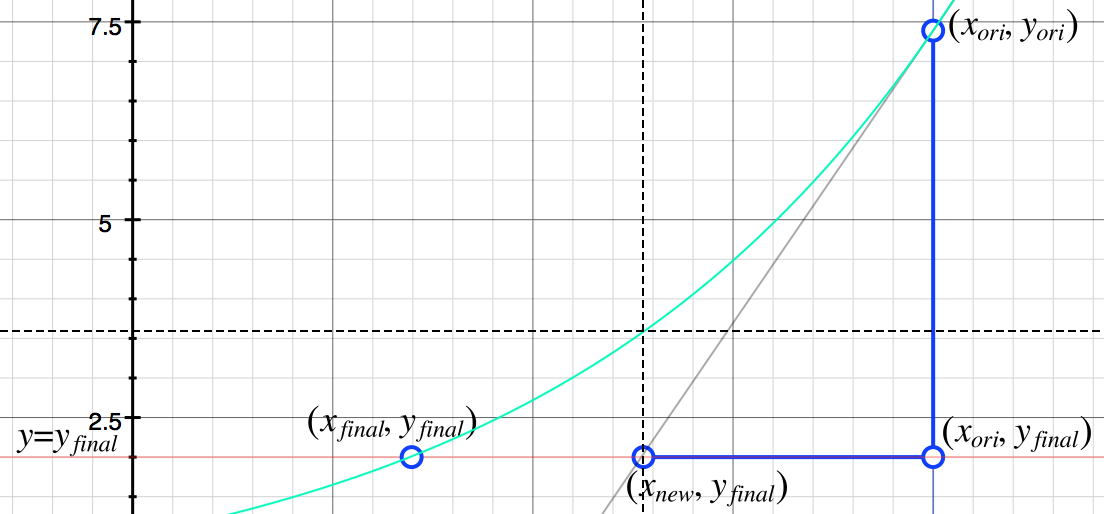
\includegraphics[scale=0.5]{images/牛顿方法示例图片}
		\caption{牛顿方法示例图}
	\end{figure}

	\item 在逻辑回归中使用牛顿方法的过程
	\begin{enumerate}
		\item 由上图可知,$\tan\alpha = \frac{y_{ori}-y_{final}}{x_{ori}-x_{new}} = \frac{f(x_{ori})-f(x_{final})}{x_{ori}-x_{new}} = f'(x_{ori})$\footnote{$\alpha$是切线$y=f'(x_{ori})x + b$与水平线$y=y_{final}$的夹角,不好标就没画出来了},可以得到
		\begin{equation}
			x_{new} := x_{ori} - \frac{f(x_{ori})-f(x_{final})}{f'(x_{ori})}
		\end{equation}
		
		\item 此时,我们得到了一个新的点$(x_{new}, y_{new})$,相比与原来的点$(x_{ori},y_{ori})$,这个点离最终的$(x_{final}, y_{final})$更近了。

		\item 特殊地,在逻辑回归中,我们要得到的是似然函数$l(\theta)$的极值,极值点的导数为$0$。于是,为了在逻辑回归中使用牛顿方法,我们用$l'(\theta)$代替$f(x)$,且$l'(\theta_{final}) = 0$,于是,上式变成
		\begin{align}
			\theta_{new} &:= \theta_{ori} - \frac{l'(\theta_{ori})-l'(\theta_{final})}{l''(\theta_{ori})} \\
			&:=  \theta_{ori} - \frac{l'(\theta_{ori})}{l''(\theta_{ori})}
		\end{align}
		这就是逻辑回归使用牛顿方法时的迭代方式
	\end{enumerate}

	\item 矩阵表达形式 \\
	将上面的式子改写为矩阵表达的形式,如下
	\begin{equation}
		\theta := \theta - H^{-1}\nabla_{\theta}l(\theta)
	\end{equation}
	其中,$H$称为Hessian\footnote{关于Hessian矩阵的介绍请见附录},是一个$n*n$矩阵
	\begin{equation}
		H_{ij} = \frac{\partial^2l(\theta)}{\partial\theta_i\partial\theta_j}
	\end{equation}

	\item 关于牛顿方法的思考
	\begin{enumerate}
		\item 因为不论我们要得到的是最大值还是最小值,其极值点的导数均为$0$,因此,虽然上述逻辑回归中,我们要得到的时似然函数的极大值,但是,若在其他问题中我们要的得到的时极小值,最终的迭代方式还是一样的。
		\item 但是,通过此方法找到的只是极值点(且每次应该只能找到一个解),很可能只是局部最优,如何保证其为全局最优(最大或最小)呢?。{\color{red}{此项待研究。。}}
	\end{enumerate}

	\item 牛顿方法与梯度下降方法的异同
	\begin{enumerate}
		\item 牛顿方法可以在很少的迭代次数就收敛,而梯度下降要收敛需要迭代的次数可能较多
		\item 但是,牛顿方法每次迭代的计算量较大(因为要计算$H^{-1}$),这在特征维度$n$较大时将会耗费较多的性能
		\item 综上,在特征维度$n$不是太大时,使用牛顿方法能够很快就收敛;但是若特征维度$n$很大时,虽然使用牛顿方法需要迭代的次数较少,但是它每次耗费的计算量太大,整个学习的时间不一定能够比梯度下降少。
	\end{enumerate}
\end{enumerate}















		\subsection{逻辑回归的代码实现 - 二分类}

\subsubsection{sigmoid函数}
\begin{equation}
	sigmoid(z) = \frac{1}{1 + e^{-z}}
\end{equation}


\subsubsection{决策函数}
\begin{enumerate}
\item 数值形式
\begin{equation}
	h_\theta(x) = \frac{1}{1 + e^{-\theta^T x}}
\end{equation}

\item 矩阵形式
\begin{equation}
	h_\theta(X) = \frac{1}{1 + e^{-X \theta}}
\end{equation}
\end{enumerate}


\subsubsection{Cost Function}
\begin{enumerate}
\item 数值形式
\begin{equation}
	J(\theta) = \frac{1}{m}
	    \sum_{i=1}^m \left[ y^{(i)}\log{h_\theta(x^{(i)})} + (1-y^{(i)})\log{(1-h_\theta(x^{(i)}))} \right]
\end{equation}

\item 矩阵形式
\begin{equation}
		J(\theta) = \frac{1}{m} \left[y^T \log{h_\theta(x)} + (1-y^T) \log{(1-h_\theta(x)}\right]
\end{equation}
\end{enumerate}

\subsubsection{偏导数$\frac{\partial J(\theta)}{\partial \theta_j}$}
\begin{enumerate}
\item 数值计算形式
\begin{equation}
	\frac{\partial J(\theta)}{\partial \theta_j} =
	    -\frac{1}{m} \sum_{i=1}^m \left[h_\theta(x^{(i)}) - y^{(i)}\right] x_j^{(i)}
\end{equation}

\item 矩阵计算形式
\begin{equation}
	\nabla J(\theta) = -\frac{1}{m} X^T \left[h_\theta(x) - y\right]
\end{equation}
\end{enumerate}


\subsubsection{梯度上升迭代算法}
\begin{enumerate}
\item 数值计算形式
\begin{equation}\begin{aligned}
	\theta_j &:= \theta_j + \alpha\frac{\partial J(\theta)}{\partial \theta_j} \\
	    &:= \theta_j - \alpha \frac{1}{m} \sum_{i=1}^m \left[h_\theta(x^{(i)}) - y^{(i)}\right] x_j^{(i)}
\end{aligned}\end{equation}

\item 矩阵计算形式
\begin{equation}\begin{aligned}
	\theta &:= \theta + \alpha\nabla J(\theta) \\
		&:= \theta - \alpha \frac{1}{m} X^T \left[h_\theta(x) - y\right]
\end{aligned}\end{equation}
\end{enumerate}


\subsection{逻辑回归的代码实现 - 多分类}
\subsubsection{使用k个分类器}
\subsubsection{使用Softmax}
% 当只有k个类别时,使用k个分类器

		
	\section{广义线性模型}
\subsection{指数分布族}
\begin{enumerate}
	\item 指数分布族的一般形式
	\begin{equation}
		p(y;\eta) = b(y)e^{\eta^T T(y) - a(\eta)}
	\end{equation}
	其中,$\eta$称为natural parameter(自然参数???); \\
	$T(y)$称为sufficient statistic(充分统计量??),大部分情况下,$T(y) = y$,在$T(y)=y$时,$\eta$往往为标量; \\
	$a(\eta)$称为 log partition function;
	\item 
\end{enumerate}

\subsection{线性回归与逻辑回归中,GLMs各部分的值}
主要是讲线性回归于逻辑回归中的式子尽可能地转化成指数分布族的一般形式,然后在根据该一般形式写出$\eta$,$T(y)$,$a(\eta)$的形式。\\
详细过程:略

\subsection{如何构造一般线性模型}




























		\subsection{Softmax Regression}
\subsubsection{关于$\phi$的说明}
\begin{enumerate}
	\item 对于总共有$k$类的分类问题,因为每个分类出现的概率和为1,故仅有$k-1$维特征是相互独立的
	\item 我们将$p(y=i;\phi)$记为$\phi_i$;于是$\phi_k=p(y=k;\phi)=1-\sum_{i=1}^{k-1}\phi_i$。
\end{enumerate}

\subsubsection{关于$T(y)$的表示法说明}
\begin{enumerate}
	\item 为了描述$T(y)$属于多分类问题中的那一类,我们用$k-1$维向量来描述$T(y)$,其中,若$T(y)$属于第$i$类,则第$i$维值为1,其余均为0\footnote{此种表示方法称为One-Hot}。示例如下:
	\begin{equation}
		T(2) = \left[\begin{matrix} 0 \\ 1 \\ 0 \\ \vdots \\ 0 \end{matrix}\right], \quad
		T(1) = \left[\begin{matrix} 1 \\ 0 \\ 0 \\ \vdots \\ 0 \end{matrix}\right], \quad 
		T(k-1) = \left[\begin{matrix} 0 \\ 0 \\ 0 \\ \vdots \\ 1 \end{matrix}\right]
	\end{equation}
	于是,$T(k)$就是个$\vec{0}$向量\footnote{因为它$0\to n-1$维均不是}
	\begin{equation}
		T(k) = \left[\begin{matrix} 0 \\ 0 \\ 0 \\ \vdots \\ 0 \end{matrix}\right]
	\end{equation}
	\item 为了描述方便,我们使用以下新的表示方法
	\begin{enumerate}
		\item $1\{\cdot\}$,在$\cdot$的值为$True$时,$1\{True\}=1$,否则$1\{False\}=0$。如$1\{2=3\}=0$,$1\{2=2\}=1$
		\item 在以上表示法下,$T(y)$可表示成以下形式
		\begin{align}
			\left(T(y)\right)_i &= 1\{y=i\} \\
			& \downarrow \\
			E\left[\left(T(y)\right)_i\right] &= P(y=i)=\phi_i
		\end{align}
	\end{enumerate}
\end{enumerate}

\subsubsection{证明多项式分布属于指数族分布}
\begin{enumerate}
	\item 在多分类问题中,$p(y;\phi)$表示的含义及其表示方式
	\begin{enumerate}
		\item 与逻辑回归时的二分类一样,$p(y=k;\phi)$表示的是取到第$k$类的概率,用$p(y;\phi)$将$p(y=1;\phi), p(y=2;\phi), \dots, p(y=k;\phi)$表示成一个表达式
		\item 参考逻辑回归的方式,我们将$p(y;\phi)$表示为
		\begin{align}
			p(y;\phi) &= \phi_{1}^{1\{y=1\}}\phi_{2}^{1\{y=2\}}\dots\phi_{k}^{1\{y=k\}} \\
			&= \phi_{1}^{1\{y=1\}}\phi_{2}^{1\{y=2\}}\dots\phi_{k}^{1-\sum_{i=1}^{k-1}1\{y=i\}} \\
			&= \phi_{1}^{\left(T(y)\right)_1}\phi_{2}^{\left(T(y)\right)_2}\dots\phi_{k}^{1-\sum_{i=1}^{k-1}\left(T(y)\right)_i} \\
			&= e^{\left(T(y)\right)_1\ln\phi_1 + \left(T(y)\right)_2\ln\phi_2 + \dots + \left(T(y)\right)_{k-1}\ln\phi_{k-1} + \left[1-\sum_{i=1}^{k-1}\left(T(y)\right)_i\right]\ln\phi_k } \\
			&= e^{\left(T(y)\right)_1\ln\frac{\phi_1}{\phi_k} + \left(T(y)\right)_2\ln\frac{\phi_2}{\phi_k} + \dots + \left(T(y)\right)_{k-1}\ln\frac{\phi_{k-1}}{\phi_k} + \ln\phi_k} \\
			&= b(y)e^{\eta^T T(y) - a(\eta)}
		\end{align}
		\end{enumerate}
	\item 从上式可得
	\begin{align}
		b(y) &= 1 \\
		\eta^TT(y) &= \left(T(y)\right)_1\ln\frac{\phi_1}{\phi_k} + \left(T(y)\right)_2\ln\frac{\phi_2}{\phi_k} + \dots + \left(T(y)\right)_{k-1}\ln\frac{\phi_{k-1}}{\phi_k} \\
		&\downarrow \\
		\eta^T &= \left[\begin{matrix}
		\ln\frac{\phi_1}{\phi_k} \\ \ln\frac{\phi_2}{\phi_k} \\ \vdots \\ \ln\frac{\phi_{k-1}}{\phi_k}
		\end{matrix}\right] \\
		a(\eta) &= -\ln\phi_k
	\end{align}
\end{enumerate}


\subsubsection{使用Softmax进行分类}
\begin{enumerate}
	\item 对于$\eta$中的某一项
	\begin{align}
		\eta_i &= \ln{\frac{\phi_i}{\phi_k}} \\
		&\downarrow \\
		e^{\eta_i} &= \phi_i \\
		&\downarrow \\
		\phi_k e^{\eta_i} &= \phi_i \\
		\phi_k\sum_{i=1}^{k}e^{\eta_i} &= \sum_{i=1}^{k}\phi_i = 1 \\
		&\Downarrow \\
		\phi_i &= \phi_k\cdot e^{\eta_i} \\
		&= e^{\eta_i} \cdot \frac{1}{\sum_{j=1}^{k}e^{\eta_j}}
	\end{align}
	如上所示,$\phi_i = \frac{e^{\eta_i}}{\sum_{j=1}^{k}e^{\eta_j}}$称为Softmax函数
	\item 最后,再使用前面的假设三:$\eta_i = \theta_i^Tx, \quad i=1,2, \dots, k-1, \quad \theta_i \in {\rm I\!R}^{n+1}$,可得到
	\begin{align}
		p(y=i|x; \theta) &= \phi_i \\
		&= \frac{e^{\eta_i}}{\sum_{j=1}^{k}e^{\eta_j}} \\ 
		&= \frac{e^{\theta_i^Tx}}{\sum_{j=1}^{k}e^{\theta_j^Tx}}
	\end{align}
	\item 故
	\begin{align}
		h_\theta(x) &= E\left[T(y)|x;\theta\right] \\
		&= E\left[\left[\begin{matrix} 1\{y=1\} \\ 1\{y=2\} \\ \vdots \\ 1\{y=k-1\} \end{matrix}\right|x;\theta\right] \\
		&= \left[\begin{matrix}\phi_1 \\ \phi_2 \\ \vdots \\ \phi_{k-1} \end{matrix}\right] \\ 
		&= \left[\begin{matrix}
		\frac{e^{\theta_1^Tx}}{\sum_{j=1}^{k}e^{\theta_j^Tx}} \\
		\frac{e^{\theta_2^Tx}}{\sum_{j=1}^{k}e^{\theta_j^Tx}} \\
		\vdots \\
		\frac{e^{\theta_{k-1}^Tx}}{\sum_{j=1}^{k}e^{\theta_j^Tx}}
		\end{matrix}\right]
	\end{align}
	如上,最终$h_\theta(x)$可得到$k-1$维向量,通过总概率为1得到第$k$维的概率值,由此可以得到每一种类别的概率值
	\item 以上得到多分类中每种分类概率值的方法就叫做Softmax回归(Softmax Regression)
\end{enumerate}


\subsubsection{参数$\theta$的拟合方式}
使用对数似然估计方法
\begin{align}
	l(\theta) &= \sum_{i=1}^{m}\ln p\left[y^{(i)}|x^{(i)};\theta\right] \\
	&= \sum_{i=1}^{m} \ln \prod_{l=1}^{k}\left[
	\frac{e^{\theta_l^Tx^{(i)}}}{\sum_{j=1}^{k}e^{\theta_l^Tx^{(i)}}}
	\right]^{1\{y^{(i)}=l\}}
\end{align}
{\color{red}{后续待补充}}













	\section{生成学习算法}
\subsection{生成学习算法简介}

\subsubsection{判别学习算法\&生成学习算法}
\begin{enumerate}
	\item 判别学习算法:计算$p(y|x)$,例如逻辑回归中计算$p(y=1|x)$与$p(y=0|x)$
	\item 生成学习算法:计算$p(x|y)$与$p(y)$,然后通过贝叶斯公式$p(y|x) = \frac{p(x|y)p(y)}{p(x)}$计算得到$p(y|x)$
	\begin{enumerate}
		\item 式子中的$p(y)$就是每个$y=k$所占的比例,既然我们有了数据,就可以用其频率当作其比例
		\item 不论$p(y|x)$中$y$的值为多少,式中的$p(x)$均是一样的值(可通过全概率公式计算得到),因此,对于$p(y|x)$较大的$y=k$,$p(x|y)p(y)$也较大,因此,在最优化过程中,可以不计算$p(x)$,于是优化过程变为
		\begin{align}
			arg\max{p(y|x)} &= arg \max_y{\frac{p(x|y)p(y)}{p(x)}} \\
			&= arg\max_y{p(x|y)p(y)}
		\end{align}
		省去了计算$p(x)$的过程
	\end{enumerate}
	
	\item 判别学习算法是给如一系列特征,得到这些特征应该是哪一种结果;生成学习算法学习的是这一种结果应该有什么特征

\end{enumerate}




















		\subsection{高斯判别分析}
以下内容中均假设$p(x|y)$服从多重正态分布(高斯分布)

\subsubsection{多重正态分布简介}
\begin{enumerate}
	\item $n$重正态分布可由均值向量$\mu \in {\rm I\!R}^n$和协方差矩阵$\Sigma \in {\rm I\!R}^{n\times n}$确定,记做$N(\mu, \Sigma)$,表示为:
	\begin{equation}
		p(x; \mu, \Sigma) = \frac{1}{(2\pi)^{\frac{n}{2}}|\Sigma|^\frac{1}{2}}e^{-\frac{1}{2}(x-\mu)^T\Sigma^{-1}(x-\mu)}
	\end{equation}
	其中,$|\Sigma|$是协方差矩阵$\Sigma$的行列式;$\Sigma=\mathrm{Cov}(X) = E(XX^T) - E(X)\left[E(X)\right]^T$,$X$的期望为$E(X) = \int_{x}xp(x;\mu,\Sigma)dx = \mu$
\end{enumerate}

\subsubsection{高斯判别分析模型}
\begin{enumerate}
	\item 高斯判别分析模型针对的是连续性随机变量,如果是离散型随机变量请使用后续会讲到的朴素贝叶斯
	\item 当我们使用高斯判别分析模型是,即有了以下的模型
	\begin{align}
		y & \sim B(1, \phi) = Bernoulli(\phi) \\
		x|y=0 &\sim N(\mu_0, \Sigma) \\
		x|y=1 &\sim N(\mu_1, \Sigma)
	\end{align}
	于是,其概率密度为:
	\begin{align}
		p(y) &= \phi^y(1-\phi)^{1-y} \\
		p(x|y=0) &= \frac{1}{(2\pi)^{\frac{n}{2}}|\Sigma|^\frac{1}{2}}e^{-\frac{1}{2}(x-\mu_0)^T\Sigma^{-1}(x-\mu_0)} \\
		p(x|y=1) &= \frac{1}{(2\pi)^{\frac{n}{2}}|\Sigma|^\frac{1}{2}}e^{-\frac{1}{2}(x-\mu_1)^T\Sigma^{-1}(x-\mu_1)}
	\end{align}
	在上式中,$\phi, \mu_0, \mu_1, \Sigma$就是我们要求的参数(注意,有2个$\mu$,共享1个$\Sigma$),其对数似然函数为:
	\begin{align}
		l(\phi, \mu_0, \mu_1, \Sigma) &= \log \prod_{i=1}^{m} p\left(x^{(i)}, y^{(i)}; \phi, \mu_0, \mu_1, \Sigma\right) \\
		&= \log \prod_{i=1}^{m} p\left(x^{(i)}|y^{(i)}; \mu_0, \mu_1, \Sigma\right)p\left(y^{(i)};\phi\right)
	\end{align}
	注意$p(x|y)$中并没有参数$\phi$,$p(y)$中只有参数$\phi$
	\item 求解似然函数后可得参数如下
	\begin{align}
		\phi &= \frac{1}{m} \sum_{i=1}^{m}1\{y^{(i)=1}\} \\
		\mu_0 &= \frac{\sum_{i=1}^{m}1\{y^{(i)}=0\}x^{(i)}}{\sum_{i=1}^{m}1\{y^{(i)}=0\}} \\
		\mu_1 &= \frac{\sum_{i=1}^{m}1\{y^{(i)}=1\}x^{(i)}}{\sum_{i=1}^{m}1\{y^{(i)}=1\}} \\
		\Sigma &= \frac{1}{m}\sum_{i=1}^{m}\left(x^{(i)}-\mu_{y^{(i)}}\right)\left(x^{(i)}-\mu_{y^{(i)}}\right)^T
	\end{align}
	下面解释下以上各参数表达式的意义: \\
	$\phi$:表示所有数据中$y=1$所占的比例; \\
	$\mu_0$: 其分母表示所有数据中$y=0$的数目,分子表示$y=0$对应的$x$的和;$\mu_1$同理 \\
	$\Sigma$: 协方差矩阵,前面已说过,不再赘述
	\item 说明
	\begin{enumerate}
		\item 使用通过高速判别分析得到的模型得到的是两个高斯分布
		\item 这两个高速分布有共同的协方差$\Sigma$,但是其期望$\mu$不一样,若画出其等高线,在图形上表现为两个等高线形状(由$\Sigma$决定)一样,但是其中心(由$\mu$决定)不一样。
	\end{enumerate}
\end{enumerate}

\subsubsection{高斯判别分析\&逻辑回归}
\begin{enumerate}
	\item 如果我们将$\phi, \mu_0, \mu_1, \Sigma$看出$x$的函数,进行整理后最终可得到
	\begin{equation}
		p(y=1|x; \phi, \mu_0, \mu_1, \Sigma) = \frac{1}{1+e^{-\theta^Tx}}
	\end{equation}
	其中,$\theta$是$\phi, \mu_0, \mu_1, \Sigma$的函数
	\item 如果$p(x|y)$服从多重高斯分布,则$p(y|x)$服从逻辑回归;但反之却不成立,从$p(y|x)$服从逻辑回归无法得到$p(x|y)$服从多重高斯分布。这说明GDA需要更多的条件,其做了更强的假设。
	\item 如果$p(x|y)$确实服从或近似服从高斯分布,那么GDA能够很好地进行预测;在数据集$m$很大时,严格意义上讲在准确率上没有比GDA更好地算法。当然,GDA会比逻辑回归好;甚至在数据集较小时,GDA也往往比逻辑回归好
	\item 因为逻辑回归的假设更弱(可理解为需要的条件更少),因此其具有更好的鲁棒性(可理解为适应能力更好),即使$p(y|x)$并不符合也不近似符合高斯分布,逻辑回归也能较好地预测
\end{enumerate}
















		\subsection{朴素贝叶斯}
\begin{enumerate}
	\item 在GDA中,随机变量$X$是连续的,当随机变量是离散值时,我们使用朴素贝叶斯来进行预测
	\item 朴素贝叶斯举例介绍:以通过邮箱中的文本预测是否为垃圾邮件为例,$y=1$表示该邮件是垃圾邮件
	\begin{enumerate}
		\item 对每封邮件建立词向量\footnote{此处的词向量比较简单,与文本分析(NLP)中的词向量不一样,也不是One-Hot的形式},每个词在向量中占据一个位置,若该词存在,则将该位的值设为1,若不存在则设为0,得到如下向量
		\begin{align}
			x = \left[\begin{matrix}1 \\ 0 \\ 0 \\ \vdots \\ 1 \\ \vdots \\ 0 \end{matrix}\right] \quad
			\begin{matrix}a \\ ad \\ address \\ \vdots \\ buy \\ \vdots \\ zygmurgy \end{matrix}
		\end{align}
		如上所示,该邮件中有a, buy等,没有ad, address, zygmurgy等。
		\footnote{一般来说,建议通过扫描训练集来获取可能出现的词(而不是从字典中获取),这样做一方面可以减小建模时的特征数,节省计算量和存储空间;另一方面还可以避免出现一些字典中没有的词(如CS299,或一些人名等)\\
		另外,还可以将一些无实意、出现频率又比较高的词去除,如a, an, the等}
		\item 若要使用多项式分布来进行预测,按照之前的逻辑回归方式,在词向量维度较多时并不可取(PS:讲义中的$2^{50000}-1$看起来似乎有问题,对$50000$个词建模只需要有$50000+1$个参数,哪来的$2^{50000}-1$??{\color{red}{待研究...}})
		\item 为了更方便地进行建模,我们做了一个假设:假设对于给定的$y$,$x_i$($x_i$指词向量中的第$i$个词)是相互条件独立的,即$p(x_2|y, x_1) = p(x_2|y)$,给定的$x_1$条件并不影响$p(x_2|y)$。此假设称为{\color{blue}{朴素贝叶斯假设}}。由此得到的分类器称为{\color{blue}{朴素贝叶斯分类器}}。
		\item 根据以上假设,我们可以得到以下式子:
		\begin{align}
			p(x_1, \dots, x_n|y) &= p(x_1|y)p(x_2|y, x_1)p(x_3|y, x_1, x_2)\dots p(x_n|y, x_1, x_2, \dots, x_{n-1}) \\
			&= p(x_1|y)p(x_2|y)p(x_3|y)\dots p(x_n|y) \\
			&= \prod_{i=1}^{n}p(x_i|y)
		\end{align}
		\item 与GDA类似,上式由参数$\phi_{i|y=1}=p(x_i=1|y=1)$,$\phi_{i|y=0}=p(x_i=1|y=0)$,$\phi_y=p(y=1)$决定。似然函数可表示为:
		\begin{align}
			L(\phi_y, \phi_{i|y=0}, \phi_{i|y=1}) = \prod_{i=1}^{n}p(x^{(i)}|y^{(i)})
		\end{align}
		\item 通过最大似然估计,可得
		\begin{align}
			\phi_{j|y=1} &= \frac{\sum_{i=1}^{m}1\{x_j^{(i)}=1 \cap y^{(i)}=1\}}{\sum_{i=1}^{m}1\{y^{(i)}=1\}} \\
			\phi_{j|y=0} &= \frac{\sum_{i=1}^{m}1\{x_j^{(i)}=1 \cap y^{(i)}=0\}}{\sum_{i=1}^{m}1\{y^{(i)}=0\}} \\
			\phi_y &= \frac{\sum_{i=1}^{m}1\{y^{(i)}=1\}}{m}
		\end{align}
		其中: \\
		$\cap$表并集,即两个条件同时满足 \\
		$\phi_{j|y=1}$表示出现词$x_j$的垃圾邮件在所有垃圾邮件中所占的比例 \\
		$\phi_{j|y=0}$表示出现词$x_j$的非垃圾邮件在所有非垃圾邮件中所占的比例 \\
		$\phi_y$表示垃圾邮件占所有邮件的比例
		\item 使用贝叶斯公式计算$p(y|x)$
		\begin{align}
			p(y=1|x) &= \frac{p(x|y=1)p(y=1)}{p(x)} \\
			&= \frac{\prod_{i=1}^{n}p(x_i|y=1)p(y=1)}{\left[\prod_{i=1}^{n}p(x_i|y=1)\right]p(y=1)+\left[\prod_{i=1}^{n}p(x_i|y=0)\right]p(y=0)}
		\end{align}
		对$p(y=0|x)$同理,通过比较那个概率更高\footnote{所以,其实$p(x)$并没有必要求,虽然也不难求}来判断是否为垃圾邮件。
		\item 虽然以上过程中只是二分类,但实际上,对于多分类也是以上的套路;
		\item 对于连续型随机变量,也可以对其分段离散化,然后使用朴素贝叶斯进行预测
	\end{enumerate}
\end{enumerate}

\subsection{拉普拉斯平滑}
\subsubsection{背景介绍}
\begin{enumerate}
	\item 在朴素贝叶斯中,若在预测时出现了一个我们训练集中没有的词,那么预测结果为
	\begin{align}
		\phi_{{x_j}|y=1} &= \frac{\sum_{i=1}^{m}1\{x_j^{(i)}=1 \cap y^{(i)}=1\}}{\sum_{i=1}^{m}1\{y^{(i)}=1\}} \\
		&= 0 \\
		\phi_{{x_j}|y=1} &= \frac{\sum_{i=1}^{m}1\{x_j^{(i)}=1 \cap y^{(i)}=0\}}{\sum_{i=1}^{m}1\{y^{(i)}=0\}} \\
		&= 0 \\
		p(y=1|x) &= \frac{\prod_{i=1}^{n}p(x_i|y=1)p(y=1)}{\left[\prod_{i=1}^{n}p(x_i|y=1)\right]p(y=1)+\left[\prod_{i=1}^{n}p(x_i|y=0)\right]p(y=0)} \\
		&= \frac{0}{0}
	\end{align}
	此时出现了$\frac{0}{0}$的情况,没法进行预测。为了解决此问题,我们可以使用拉普拉斯平滑。\footnote{吴恩达的视频中,举了一个已知前面5次比赛都失败,预测第6次失败的概率,可以看下。}
\end{enumerate}

\subsubsection{拉普拉斯平滑介绍}
\begin{enumerate}
	\item $\frac{0}{0}$出现的原因 \\
	由前面$\phi_j = \frac{\sum_{i=1}^{m}1\{z^{(i)}=j\}}{m}$可知,$\phi_j$为出现$z^{(i)}=j$的数据占总数据的比例,在$z^{(i)}=j$在训练集中未出现过时,就会出现$\phi_j=0$\footnote{在$=0$处频数为0,在$=1$处频数也为0},从而导致出现$\frac{0}{0}$的情况,为了解决此问题,我们队$\phi_j$稍作更改:
	\begin{equation}
		\phi_j = \frac{\sum_{i=1}^{m}1\{z^{(i)}=j\}+1}{m+k}
	\end{equation}
	经过此方式处理后:
	\begin{enumerate}
		\item $\sum_{j=1}^{k}\phi_j = 1$仍旧成立
		\item 对任意$\phi_j \neq 0$
	\end{enumerate}
\end{enumerate}














		\subsection{文本分类}
\begin{align}
	\phi_{k|y=1} &= \frac{\sum_{i=1}^{m}\sum_{j=1}^{n}1\{x_j^{(i)}=k \cap y^{(i)}=1\}+1}{\sum_{i=1}^{m}1\{y^{(i)}=1\}n_i + |V|} \\
	\phi_{k|y=0} &= \frac{\sum_{i=1}^{m}\sum_{j=1}^{n}1\{x_j^{(i)}=k \cap y^{(i)}=0\}+1}{\sum_{i=1}^{m}1\{y^{(i)}=0\}n_i + |V|}
\end{align}


详情略, 待补充









	\section{支持向量机}

\subsection{逻辑回归的缺陷}
\begin{enumerate}
	\item 按照逻辑回归的计算方式,我们得到的是一个分隔线(或平面或超平面\footnote{1维称为线,2维称为平面,更多维就称为超平面}),对于我们的数据点,总有一些点离超平面较近(如点C),有一些点离超平面较远(如点A);对于离超平面较远的点,我们有很大把握保证我们的预测是准确的,但是,对于离超平面较近的点我们就没把握了。
	\begin{figure}[htbp]
		\centering
		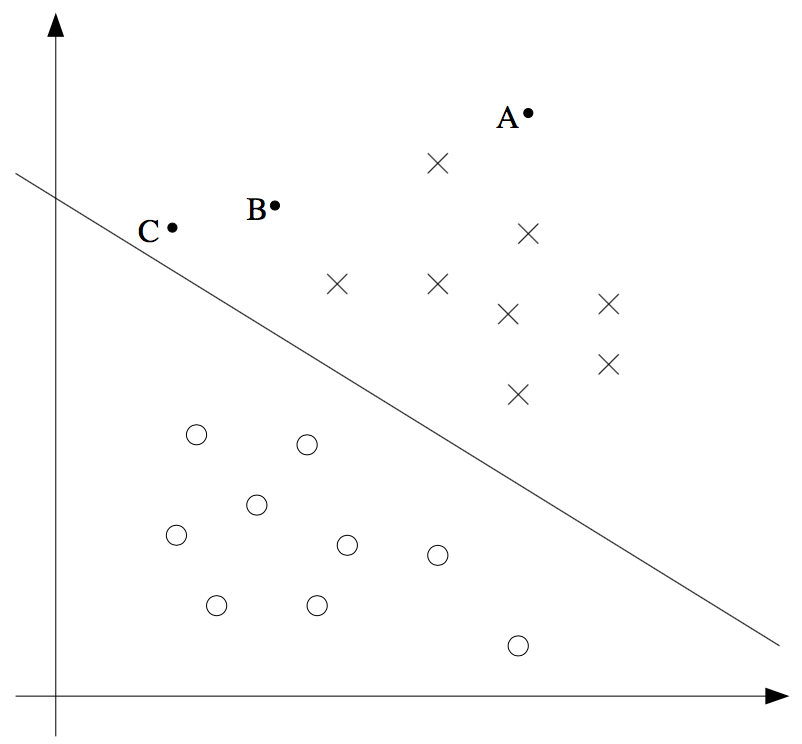
\includegraphics[scale=0.5]{images/逻辑回归缺陷讲述}
	\end{figure}
\end{enumerate}

\subsection{SVM前言}
\begin{enumerate}
	\item 在后续介绍SVM过程中,为了描述方便,我们对之前逻辑回归的一些描述做了更改
	\item 将$h_\theta(x)$更改为$h_{w,b}(x)$,其中:$w \to \left[\begin{matrix}\theta_1 \\ \theta_2 \\ \vdots \\ \theta_n  \end{matrix}\right]$,$b \to \theta_0$\footnote{此处为了表达方便,使用$\to$来表达类似的对应关系,且勿将其当做等于"$=$"}
	\item 将类标签$y$改为$\{-1, 1\}$;将$h=g(w^T+b)$的值从值域$\{0,1\}$切换到$\{-1, 1\}$,其中,$0\to -1$,$1\to 1$
	,且取消原有的$x_0=1$假设。通过此方式将$h(x)$由参数$\theta$变成了参数$(w, b)$,将截距项$b$与其他项分隔开,以便分析
\end{enumerate}

\subsection{Margin介绍}
\subsubsection{函数间隔}
\begin{enumerate}
	\item 对于数据点$(x^{(i)}, y^{(i)})$,其函数间隔定义为:
	\begin{align}
		\hat{\gamma}^{(i)} = y^{(i)}(w^Tx^{(i)} + b)
	\end{align}
	\item 对于$y^{(i)}=1$的点,为了让函数间隔$\hat{\gamma}$越大,我们需要让$w^Tx^{(i)} + b$正向越大;
	\item 对于$y^{(i)}=-1$的点,为了让函数间隔$\hat{\gamma}$越大,我们需要让$w^Tx^{(i)} + b$负向越大;
	\item 对于给定的训练集$S=\{(x^{(i)}, y^{(i)}); \quad i = 1, \dots, m\}$,我们将其中最小的函数间隔记为$\hat{\gamma}$:
	\begin{align}
		\hat{\gamma} = \min_{i=1,\dots,m}\hat{\gamma}^{(i)}
	\end{align}
	\item 对于函数间隔,若将参数$(w,b)$扩大2倍2为$(2w,2b)$,函数间隔的值$\hat{h}_{w,b}(x)$也变成了原来的2倍,但实际上,这对训练的效果并没有影响,原来错误的现在还是错误
\end{enumerate}

\subsubsection{几何间隔}
\begin{enumerate}
	\item 几何间隔表示为$\gamma^{(i)}$\footnote{与函数间隔相比,少了头顶的帽子: $\hat{ }$}。
	\item 对于数据点$(x^{(i)}, y^{(i)})$,其几何间隔定义为\footnote{证明过程略}:
	\begin{align}
		\gamma^{(i)} &= \frac{\hat{\gamma}^{(i)}}{\|w\|}  \\
		&= \frac{y^{(i)}(w^Tx^{(i)} + b)}{\|w\|}  \\
		&=  y^{(i)} \left(\left(\frac{w}{\|w\|}\right)^T x^{(i)} + \frac{b}{\|w\|}\right)
	\end{align}
	\item 当$\|w\|=1$时,几何间隔与函数间隔相等
	\item 相较于函数间隔,几何间隔任意缩放参数$(w,b)$不影响$h_{w,b}(x)$的值;鉴于此性质,我们可以在训练时对$w, b$视需求进行缩放
	\item 同样,对于给定的训练集$S=\{(x^{(i)}, y^{(i)}); \quad i = 1, \dots, m\}$,我们将其中最小的几何间隔记为$\gamma$:
	\begin{align}
		\gamma = \min_{i=1,\dots,m}\gamma^{(i)}
	\end{align}
\end{enumerate}

\subsubsection{函数间隔\&几何间隔}
\begin{enumerate}
	\item 当预测正确时,二者都是正值;当预测错误是,二者都是负值。
\end{enumerate}























		\subsection{最优间隔分类器-优化目标}
\subsubsection{将难以优化的目标转为容易优化的}
\begin{enumerate}
	\item 通过前面的讲述我们知道,为了对给定的数据集进行分类,我们需要找到使得几何间隔最大化的决策边界(在下面的讲述中,先假设我们会遇到的数据集都是线性可切分的,等我们讲到核函数时再去除这个假设)。于是,可以用以下的式子来描述我们要优化的目标
	\begin{align}
		\max_{\gamma, w, b} \gamma
	\end{align}
	根据前面的定义:$\gamma = \min_{i=1,\dots,m}\gamma^{(i)}$,$\gamma$是所有数据点中几何间隔最小值,所以,对于任意数据点,其几何间隔均应大于$\gamma$\footnote{这是约束条件,请注意优化目标与约束条件的差别。}:
	\begin{align}
		y^{(i)}\frac{(w^Tx^{(i)}+b)}{\|w\|} \geq \gamma, \quad i=1, 2, \dots, m
	\end{align}
	因为对于几何间隔,缩放$w$或$b$或都缩放不会影响决策边界的位置\footnote{决策边界始终由$w^Tx^{(i)}+b=0$确定},于是,我们定义$\|w\|=1$,让几何间隔与函数间隔相等,于是:
	\begin{align}
		&\text{优化目标:} \\
		& \qquad \max_{\gamma, w, b} \gamma \\
		&\text{约束条件:} \\
		& \qquad y^{(i)}(w^Tx^{(i)}+b) \geq \gamma, \quad i=1, 2, \dots, m \\
		& \qquad \|w\| = 1
	\end{align}

	\item 经过上面的转化后,$\|w\|=1$这个约束还是不好处理,我们需要想办法去除这个约束,于是将优化目标$\gamma$改写为$\frac{\hat{\gamma}}{\|w\|}$\footnote{课上有人问为什么要使用函数间隔?为什么要对它除以$\|w\|$?实际上$\frac{\hat{\gamma}}{\|w\|}$只是$\gamma$的另一种表述,为了后续消去不好处理的约束$\|w\| = 1$才这样处理的。}:
	\begin{align}
		\max_{\gamma, w, b} \frac{\hat{\gamma}}{\|w\|}
	\end{align}
	约束条件变为:
	\begin{align}
		y^{(i)}\frac{(w^Tx^{(i)}+b)}{\|w\|} \geq \frac{\hat{\gamma}}{\|w\|}, \quad i=1, 2, \dots, m
	\end{align}
	消去$\|w\|$,得:
	\begin{align}
		&\text{优化目标:} \\
		& \qquad \max_{\gamma, w, b} \frac{\hat{\gamma}}{\|w\|} \\
		&\text{约束条件:} \\
		& \qquad y^{(i)}(w^Tx^{(i)}+b) \geq \hat{\gamma}, \quad i=1, 2, \dots, m
	\end{align}
	如上,经过这样的转化,我们将$\|w\|$消掉了,同时$\|w\| = 1$的假设也可以取消了。

	\item 我们令$\hat{\gamma}=1$\footnote{这样做是合理的,因为不论$\hat{\gamma}$取何值,我们都可以通过缩放$\|w\|$来消除实际的$\hat{\gamma}$与$\hat{\gamma}=1$的差距}\footnote{有的地方会将两条经过支持向量的直线标记为$w^Tx+b=1$和$w^Tx+b=-1$,这是正确的,因为,函数间隔中,$y^{(i)}$的作用只是改变函数间隔$\hat{\gamma}$的正负号,而支持向量对应的就是函数间隔为1的点,代入后就可以得到这两条直线的方程},于是优化目标变成:
	\begin{align}
		\max_{\gamma, w, b} \frac{1}{\|w\|}
	\end{align}
	最大化$\frac{1}{\|w\|}$也即最小化$\|w\|$,即最小化$\|w\|^2$,故:
	\begin{align}
		&\text{优化目标:} \\
		& \qquad \min_{\gamma, w, b} \frac{1}{2}\|w\|^2 \\
		&\text{约束条件:} \\
		& \qquad y^{(i)}(w^Tx^{(i)}+b) \geq 1, \quad i=1, 2, \dots, m
	\end{align}
\end{enumerate}




































		\subsection{拉格朗日对偶规划}
\subsubsection{拉格朗日乘数法}
\begin{enumerate}
	\item 在等式约束下求最优问题求解中可使用拉格朗日乘数法,其要解决的问题可表述如下:
	\begin{align}
		&\text{优化目标:} \\
		& \qquad \min_{w} f(w) \\
		&\text{约束条件:} \\
		& \qquad h_i(w) = 0, \quad i=1,\dots,l
	\end{align}
	$l$是等式约束的个数
	\item 其拉格朗日函数为:
	\begin{align}
		\mathcal{L}(w,\beta) = f(w) + \sum_{i=1}^{l}\beta_ih_i(w)
	\end{align}
	\item 求拉格朗日函数的偏导数
	\begin{align}
		\frac{\partial \mathcal{L}}{\partial w_i} &= 0\\
		\frac{\partial \mathcal{L}}{\partial \beta_i} &= 0
	\end{align}
	求解上式,得到$w, \beta$即可
\end{enumerate}

\subsubsection{拉格朗日对偶规划}
\begin{enumerate}
	\item 对于有不等约束的问题,拉格朗日乘数法就无能为力了;这时就需要用拉格朗日对偶规划,其所要解决的问题可表述如下:
	\begin{align}
		&\text{优化目标:} \\
		& \qquad \min_{w} f(w) \\
		&\text{约束条件:} \\
		& \qquad g_i(w) \leq 0, \quad i=1,\dots,k \\
		& \qquad h_i(w) = 0, \quad i=1,\dots,l
	\end{align}
	$k, l$为对应约束的个数。\\
	称其为原问题。
	\item 其generalized Lagrangian\footnote{{\color{red}{不知道怎么翻译}}}为:
	\begin{align}
		\mathcal{L}(w, \alpha, \beta) = f(w) + \sum_{i=1}^{k}\alpha_ig_i(w) + \sum_{i=1}^{l}\beta_ih_i(w)
	\end{align}
	\item 下面我们定义以下式子:
	\begin{align}
		\theta_{\mathcal{P}}(w) = \max_{\alpha, \beta; \alpha_i\geq0} \mathcal{L}(w, \alpha, \beta)
	\end{align}
	注意,在上面的式子中,我们对$\alpha_i$做了限制:$\alpha_i\geq 0$,于是,$\theta_{\mathcal{P}}(w)$便有了以下性质:
	\begin{enumerate}
		\item 当$g_i(w)$不满足约束条件,即$g_i(w)>0$时,为了使$\mathcal{L}(w, \alpha, \beta)$取到更大,我们只需要让$\alpha_i$更大就行,很显然,此时$\max \mathcal{L}(w, \alpha, \beta) = +\infty = \theta_{\mathcal{P}}(w)$
		\item 当$h_i(w)$不满足约束条件时,即$h_i(w)>0$或$h_i(w)<0$,我们同样只需要更改$\beta_i$的值就能让$\max \mathcal{L}(w, \alpha, \beta)$取到$+\infty$
		\item 当$g_i(w)$与$h_i(w)$均满足约束条件时,$\sum_{i=1}^{k}\alpha_i g_i(w)$的最大值是0;$\sum_{i=1}^{l}\beta_ih_i(w)$始终为0;所以,$\theta_{\mathcal{P}}(w)=\max_{\alpha, \beta; \alpha_i\geq0} \mathcal{L}(w, \alpha, \beta)=f(w)$
		\item 综上,我们可以得到以下式子:
		\[ \theta_{\mathcal{P}}(w)=\begin{cases}
		f(w) \quad \text{符合所有约束条件} \\
		+\infty \quad \text{其他}
		\end{cases} \]
	\end{enumerate}

	\item 通过上面的式子我们可以知道,在满足所有约束条件的情况下,$f(w)=\theta_{\mathcal{P}}(w)$,求解$f(w)$的最小值就等同于求解$\theta_{\mathcal{P}}(w)$的最小值,于是我们的优化目标就变成了:
	\begin{align}
		\min_{w} \max_{\alpha, \beta; \alpha_i \geq 0} \mathcal{L}(w, \alpha, \beta)
	\end{align}
	注意:
	\begin{enumerate}
		\item 对于$\min_{w}$,这是由我们的优化目标$\min_{w}f(w)$带来的
		\item $\max_{\alpha, \beta; \alpha_i \geq 0} \mathcal{L}(w, \alpha, \beta)$是一个整体,此式子表示的是取得$\mathcal{L}(w, \alpha, \beta)$的最大值的最小值
	\end{enumerate}

	\item 相对于前面的求拉格朗日函数最大值$\theta_{\mathcal{P}}(w) = \max_{\alpha, \beta; \alpha_i\geq0} \mathcal{L}(w, \alpha, \beta)$,其{\color{blue}{对偶问题}}\footnote{为什么要讲到其对偶问题呢?后面会讲到。}为求拉格朗日函数的最小值:
	\begin{align}
		\theta_{\mathcal{D}}(\alpha, \beta) = \min_{w} \mathcal{L}(w, \alpha, \beta)
	\end{align}
	对偶问题对应的{\color{blue}{对偶优化问题}}为:
	\begin{align}
		\max_{\alpha, \beta;\alpha_i \geq 0} \theta_{\mathcal{D}}(\alpha, \beta) = \max_{\alpha, \beta;\alpha_i \geq 0} \min_{w} \mathcal{L}(w, \alpha, \beta)
	\end{align}
	\footnote{注意,这个对偶优化问题并不是我们推导出来的,可以说是我们为了后续需要设计出来的,所以不要去想为什么这个式子是这样子的了。}

	\item 对比一下原问题与其对偶问题,可以发现,两者之间的差别只是对调了求最大值$\max_{\alpha, \beta;\alpha_i \geq 0}$与最小值$\min_{w}$的顺序。在后面的描述中,我们用$p^{*}$表示原问题的最优解,用$d^{*}$表示对偶问题的最优解:
	\begin{align}
		p^{*} &= \min_{w} \max_{\alpha, \beta; \alpha_i \geq 0} \mathcal{L}(w, \alpha, \beta) \\
		d^{*} &= \max_{\alpha, \beta;\alpha_i \geq 0} \min_{w} \mathcal{L}(w, \alpha, \beta)
	\end{align}

	\item 原问题与其对偶问题有以下性质:
	\begin{align}
		d^{*} = \max_{\alpha, \beta;\alpha_i \geq 0} \min_{w} \mathcal{L}(w, \alpha, \beta) \leq 
		\min_{w} \max_{\alpha, \beta; \alpha_i \geq 0} \mathcal{L}(w, \alpha, \beta) = p^{*}
	\end{align}
	在一些特定条件(KKT条件)下,取等号。这时,就可以将原优化问题转化为对偶优化问题求解了。

	\item KKT条件 \\
	假设$f(w), g_i(w)$是凸函数、$h_i(w)$是仿射函数、存在$w$使得$g_i(w) < 0$对所有的$i$都成立,那么一定会存在$w^*, \alpha^*, \beta^*$\footnote{其中$w^*$是原问题的解,$\alpha^*, \beta^*$是对偶问题的解,且$p^*=d^*=\mathcal{L}(w^*, \alpha^*, \beta^*)$}满足以下条件:
	\begin{align}
		\frac{\partial\mathcal{L}(w^*, \alpha^*, \beta^*)}{\partial w_i} &= 0, \quad i=1, \dots, n \\
		\frac{\partial\mathcal{L}(w^*, \alpha^*, \beta^*)}{\partial \beta_i} &= 0, \quad i=1, \dots, l \\
		\alpha_i^*g_i(w^*) &= 0, \quad i=1, \dots, k \\
		g_i(w^*) &\leq 0, \quad i=1, \dots, k  \\
		\alpha^* &\geq 0, \quad i=1, \dots, k 
	\end{align}
	其中:\\
	$\alpha_i^*g_i(w^*) = 0, \quad i=1, \dots, k$称为KKT对偶互补条件;当$\alpha^* > 0$时,$g_i(w^*) = 0$。后续会用到此性质。
\end{enumerate}
本部分内容参考资料:\url{http://blog.csdn.net/Victor_Gun/article/details/45227999}









































		\subsection{最优间隔分类器-优化方法}
\begin{enumerate}
	\item 根据前面推导出来的优化目标及拉格朗日对偶规划的内容,我们可以得到不等式约束为:
	\begin{align}
		g_i(w) = -y^{(i)}\left(w^Tx^{(i)}+b\right)+1 \leq 0
	\end{align}
	在此问题中,没有等式约束。\\
	由前面提到的KKT对偶互补条件可知,当且仅当$g_i(w)=0$时,$\alpha_i$可以不为0。令$g_i(w)=0$的点就是几何间隔$=1$的点,即与决策边界最靠近的点\footnote{在我们前面的推导过程中,有让几何间隔$=1$,所以这些点就是离决策边界最近的点},这些点称为支撑向量(Support Vectors),如下图3个红框标识的点:
	\begin{figure}[htbp]
		\centering
		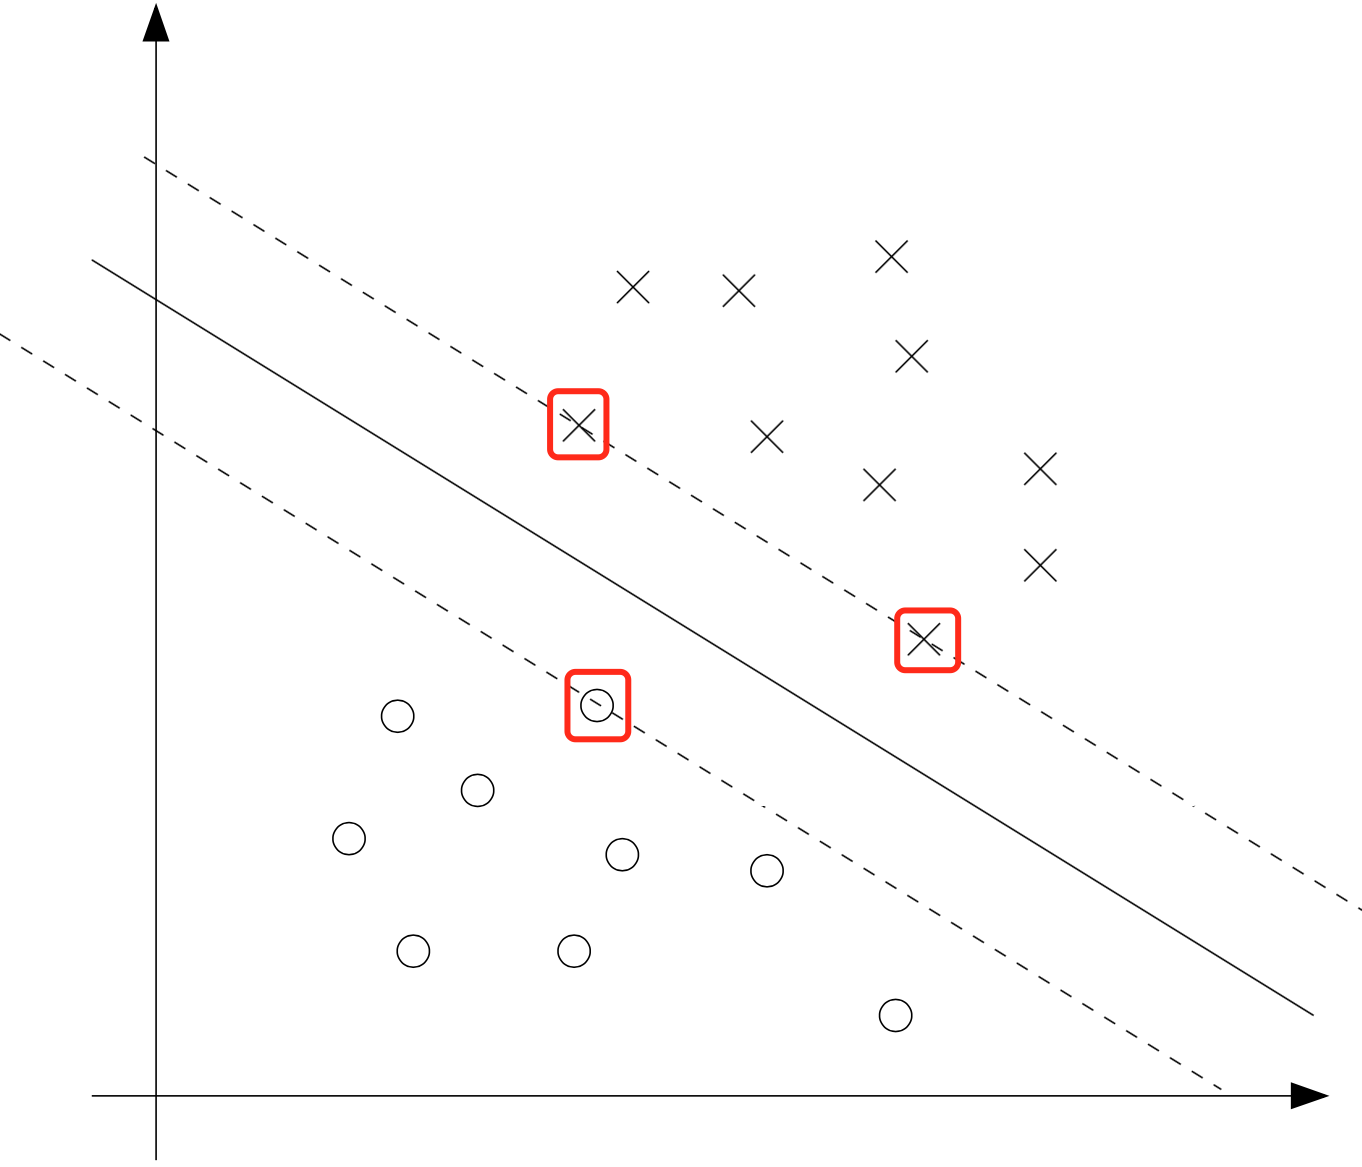
\includegraphics[scale=0.35]{images/支撑向量}
		\caption{支撑向量}
	\end{figure}

	\item 拉格朗日函数为:
	\begin{align}
		\mathcal{L}(w, b, \alpha) = \frac{1}{2}\|w\|^2 - \sum_{i=1}^{m}\alpha_i \left[y^{(i)}(w^Tx^{(i)}+b)-1\right]
	\end{align}
	注意,因为在我们的问题中没有等式约束,故上式没有$\beta_i$。

	\item 接下来我们对拉格朗日函数求偏导数,令偏导数的值为0。
	\begin{align}
		\nabla_{w}\mathcal{L}(w,b,\alpha)=w - \sum_{i=1}^{m}\alpha_iy^{(i)}x^{(i)}=0
	\end{align}
	可得:
	\begin{align}
		w = \sum_{i=1}^{m}\alpha_iy^{(i)}x^{(i)}
		\label{$w$}
	\end{align}
	对$b$:
	\begin{align}
		\frac{\partial}{\partial b}\mathcal{L}(w,b,a) = \sum_{i=1}^{m}a_iy^{(i)}=0
		\label{b}
	\end{align}
	将\ref{$w$}代入拉格朗日函数,得:
	\begin{align}
		\mathcal{L}(w,b,\alpha) = \sum_{i=1}^{m}\alpha_i-\frac{1}{2}\sum_{i,j=1}^{m}y^{(i)}y^{(j)}\alpha_i\alpha_j (x^{(i)})^Tx^{(j)} - b\sum_{i=1}^{m}a_iy^{(i)}
	\end{align}
	再将\ref{b}代入上式,得到:
	\begin{align}
		\mathcal{L}(w,b,\alpha) = \sum_{i=1}^{m}\alpha_i-\frac{1}{2}\sum_{i,j=1}^{m}y^{(i)}y^{(j)}\alpha_i\alpha_j (x^{(i)})^Tx^{(j)}
	\end{align}
	\item 下面我们考虑原问题的对偶优化问题,即:
	\begin{align}
		&\text{优化目标:} \\
		& \qquad \max_{\alpha} W(\alpha) = \sum_{i=1}^{m}\alpha_i-\frac{1}{2}\sum_{i,j=1}^{m}y^{(i)}y^{(j)}\alpha_i\alpha_j \langle x^{(i)}, x^{(j)}\rangle \\
		&\text{约束条件:} \\
		& \qquad \alpha_i \geq 0, \quad i=1,\dots,m \\
		& \qquad \sum_{i=1}^{m}\alpha_iy^{(i)} = 0
	\end{align}
	其中,$\langle x^{(i)}, x^{(j)}\rangle $表示内积\\
	第一个约束是我们一直有的,第二个约束通过求$b$的偏导数后得到\footnote{吴恩达在视频中解释这个约束说明的意义:若$\sum_{i=1}^{m}\alpha_iy^{(i)} \neq 0$,则$\theta_{\mathcal{D}}(\alpha)=-\infty$,所以,如果我们要$\max \theta_{\mathcal{D}}(\alpha)$,就应该取那些能让$\sum_{i=1}^{m}\alpha_iy^{(i)} = 0$的$\alpha$,这样,$\theta_{\mathcal{D}}(\alpha)=W(\alpha)$。{\color{red}{我也没怎么懂,待后面研究研究}}}。

	\item 若要得到$w$,根据公式\ref{$w$},我们可以知道,只要求得了$\alpha$就能得到$w$

	\item 在开始计算前,我们再仔细看下公式\ref{$w$},$w$是关于$\alpha$的函数,我们将其代入$w^Tx+b$后可以发现:
	\begin{align}
		w^Tx + b &= \left( \sum_{i=1}^{m}\alpha_i y^{(i)}x^{(i)} \right)^Tx + b \\
		&= \sum_{i=1}^{m}\alpha_iy^{(i)}\langle x^{(i)}, x \rangle + b \\
		&\downarrow	\\
		h_{w,b}(x) &= g(w^Tx + b) \\
		&= g(\sum_{i=1}^{m}\alpha_iy^{(i)}\langle x^{(i)}, x \rangle + b)
	\end{align}
	前面我们已经讨论过了,除了支撑向量对应的那几个点之外,其余的点$\alpha_i$均为0,而支撑向量的数目很少,这将大大简化我们的计算。

	\item 假设我们已经得到了$w^*$,我们便得到了一堆的平行线(因为决策边界只剩截距$b$不知道了),我们自然会取两类点中间的直线,这样才能保证离每一类都最远,于是:
	\begin{align}
		b^* = - \frac{\max_{i;y^{(i)}=-1}w^*x^{(i)} + \max_{i;y^{(i)}=1}w^*x^{(i)}}{2}
	\end{align}


\end{enumerate}


















		\subsection{核}
为方便后续内容的理解,我先大体讲一下下面的内容: \\

在我们碰到的问题中,有些在低维下不是线性可分的,但是其在高维下却是线性可分的,于是,我们可以将低维下的特征映射到高维中,然后再高维下进行分割,这里的从低维映射到高维就是的方法就是我们后面会提到的$\phi(x)$;但是,这又会带来一个问题,那就是,映射到高维后,如果仅仅制作映射而不做其他优化,我们计算的时间复杂度就上去了,于是我们就想办法来对计算方法进行改善,这个改善的方法就是使用核函数!通过使用核函数,我们并不需要知道我们从低维映射到高维到底是如何映射的(即我们并不显示地知道$\phi(x)$长什么样,我们只知道通过核函数可以达到与通过$\phi(x)$映射后一样的结果)。 \\

简而言之,引出$\phi(\cdot)$是为了说明低维不可分割的数据在高维可能可以分割;再举一堆例子说明通过得到$\phi(\cdot)$后再求$\phi(\cdot)$内积的方式计算量太大,不可取,有更好的计算方式,那就是使用核函数$K(x, z)$\\

按我个人的经验,吴恩达的视频在你还搞不明白核函数的内容时都听不懂他在讲什么,但是在搞明白后就觉得讲得很清晰(也不排除我没认真听......),可以先参考下下面的这篇博文:\url{http://blog.pluskid.org/?p=685} \\

下面开始正文

\subsubsection{特征映射与核函数引入}
\begin{enumerate}
	\item 在前面的线性回归中,我们提到,为了得到更好的拟合结果,我们可以添加高阶项如$x^2, x^3$等来优化拟合结果。为了区分远有的$x$,以及我们添加的$x^2, x^3, ...$,我们将原有的$x$称为问题的{\color{blue}{属性}},将新添加的$x^2, x^3,...$以及$x$一起称为问题的{\color{blue}{特征}}。从$x \to \left[\begin{matrix}x \\ x^2 \\ x^3\end{matrix}\right]$称为特征映射。记为$\phi$,如本例子中:$\phi(x) = \left[\begin{matrix}x \\ x^2 \\ x^3\end{matrix}\right]$

	\item 在前面的算法中,我们可以将内积$\langle x, z \rangle$改为$\langle \phi(x), \phi(x) \rangle$,我们将其定义为高斯函数:
	\begin{align}
		K(x, z) = \phi(x)^T \phi(z)
	\end{align}

	\item 但是,在映射后$\phi(x)^T \phi(z)$的计算量太大,比如
	\begin{enumerate}
		\item 我们先定义一个核函数$K(x, z)=(x^T z)^2$,然后找出其特征映射$\phi(x)$,以此说明若要显式地写出$\phi(x)$的式子与只知道核函数不使用显式的$\phi(x)$两者间的计算量差异。
		\item 对$K(x, z)$进一步计算
		\begin{align}
			K(x, z) &= \left(\sum_{i=1}^{n}x_iz_i \sum_{j=1}^{n}x_jz_j \right) \\
			&= \sum_{i=1}^{n} \sum_{j=1}^{n} x_i x_j z_i z_j \\
			&= \sum_{i,j=1}^{n}(x_i x_j) (z_i z_j)
		\end{align}
		如上,以$n=3$为例,若要将$K(x, z)$表示成$\phi(x)^T\phi(z)$的形式:
		\begin{align}
			\phi(x) = \left[\begin{matrix}x_1 x_1 \\ x_1 x_2 \\ x_1 x_3 \\ x_2 x_1 \\ x_2 x_2 \\ x_2 x_3 \\ x_3 x_1 \\ x_3 x_2 \\ x_3 x_3 \\\end{matrix}\right]
		\end{align}
		$\phi(z)$同理。显然,在上面的$\phi(x)$中,若要讲$x \to \phi(x)$,我们需要进行9次的计算;
		\item 但是,若我们不管$\phi(x)$应如何表示,直接先计算$x^Tz$后再取平方,$n=3$时只需要计算3次。
		\item 实际上,此处的$K(x, z) = (x^T z)^2$ 是我们后面会讲到的多项式核$K(x,z)=\left(\langle x, z \rangle +R \right)^d = \left(x^Tz +R\right)^d$的一种。虽然核函数$K(x,z)$可以很容易地表示出来,但是其特征映射$\phi(x)$却不见得容易表示。
	\end{enumerate}

	\item 所以,虽然前面使用将$x$映射到高维$\phi(x)$来说明这样做可以将低维无法线性分隔的点分隔开,但是在实际计算中,我们并不会去计算$\phi(x)$应如何表示,相当于我们实际上使用更容易计算的核函数$K(x, z)$来达到特征映射$\phi(x)$将低维映射到高维的效果

	\item 我们会做的是找到一个核函数,证明它确实对应着存在一个特征映射$\phi(x)$可以实现将数据在高维特征下分割开。

	\item 注: 下面说明下\url{http://blog.pluskid.org/?p=685}中的例子应如何理解
	\begin{enumerate}
		\item 例子中说明提到:$\phi(\cdot)$的目的是使得向量$x_1=(\eta_1, \eta_2)^T, x_2=(\xi_1, \xi_2)^T$在经过$\phi(\cdot)$映射后再求内积的结果为:
		\begin{align}
			\langle \phi(x_1), \phi(x_2) \rangle = \eta_1\xi_1 + \eta_1^2\xi_1^2 + \eta_2\xi_2 + \eta_2^2\xi_2^2 + \eta_1\eta_2\xi_1\xi_2
		\end{align}
		\item 但是,若我们不知道$\phi(\cdot)$是何种形式,直接通过某个核函数$K(x_1, x_2)$也可以得到同样的结果:
		\begin{align}
			\left( \langle x_1, x_2 \rangle +1 \right)^2 &= \langle x_1, x_2 \rangle ^2 + 2 \langle x_1, x_2 \rangle + 1 \\
			&= (x_1^T x_2)^2 + 2x_1^T x_2 + 1 \\
			&=\left\{ \left[\begin{matrix}\eta_1 & \eta_2\end{matrix}\right]\left[\begin{matrix}\xi_1 \\ \xi_2\end{matrix}\right] \right\}^2 + 2\left[\begin{matrix}\eta_1 & \eta_2\end{matrix}\right]\left[\begin{matrix}\xi_1 \\ \xi_2\end{matrix}\right] + 1 \\
			&= (\eta_1\xi_1+\eta_2\xi_2)^2 + 2(\eta_1\xi_1+\eta_2\xi_2) + 1 \\
			&= \eta_1^2\xi_1^2 + \eta_2^2\xi_2^2 + 2\eta_1\eta_2\xi_1\xi_2 + 2\eta_1\xi_1 + 2\eta_2\xi_2 + 1 \\
		\end{align}
		与前面的式子相比,只要对某些维度进行线性缩放即可,说明两者可以达到同样的效果。
		\item 但是,在计算量上,用第一种方法我们需要先找到其对应的$\phi(\cdot)$(若$\phi(x_1, x-2)=(\sqrt{2}x_1, x_1^2, \sqrt{2}x_2, x_2^2, \sqrt{2}x_1x_2, 1)^T$则可得到与$\left( \langle x_1, x_2 \rangle +1 \right)^2$一样的结果),然后再计算$\phi(\cdot)$的内积。显然,通过$\phi(\cdot)$的方式计算量太大,但是使用核函数计算的方式计算量就小多了。这就是该例子的目的
	\end{enumerate}

	\item 对$\phi(\cdot)$的一个直观但可能不是太准确的描述:对于$\phi(x)$和$\phi(z)$,如果两者比较相近,则其核函数$K(x,z)=\phi(x)^T\phi(z)$值较大;若干两者相差较远,则其结果值较小。所以我们可以将核函数$K(x,z)$看成是对$x,z$有多相近的一种表示。
\end{enumerate}

\subsubsection{常用核函数介绍}
\begin{enumerate}
	\item 多项式核
	\begin{align}
		K(x_1, x_2) = \left(\langle x_1, x_2 \rangle + R\right)^d
	\end{align}
	\item 高斯核
	\begin{align}
		K(x_1, x_2) = e^{-\frac{\|x_1 - x_2\|^2}{2\sigma^2}}
	\end{align}
	高斯核会将原始空间映射到无穷维空间。如果$\sigma$选得很大,高次特征上得权重就衰减得非常快,类似于一个低维的子空间;若$\sigma$选得很小,则可将任意的数据映射为线性可分,不过这可能会带来严重的过拟合问题。\\
	通过调整参数$\sigma$,高斯核具有很高的灵活性,它也是使用最广泛的核函数之一。
	\item 线性核
	\begin{align}
		K(x_1, x_2) = \langle x_1, x_2 \rangle
	\end{align}
	这实际上就是原始空间上的内积。
\end{enumerate}

\subsubsection{核函数需要满足的条件}
\begin{enumerate}
	\item 核矩阵
	对于一个有$\{x^{(1)}, x^{(2)}, \dots, x^{(m)}\}$个数据点的数据集,我们定义核矩阵中的某一项$K_{ij}$为:
	\begin{align}
		K_{ij} = K(x^{(i)}, x^{(j)})
	\end{align}
	核矩阵是一个$m\times m$矩阵
	\item 如果$K$是一个满足条件的(合法的)核函数,则
	\begin{align}
		K_{ij} = K(x^{(i)}, x^{(j)}) = \phi(x^{(i)})^T\phi(x^{(j)}) = \phi(x^{(j)})^T\phi(x^{(i)}) = K(x^{(j)}, x^{(i)}) = K_{ji}
	\end{align}
	所以说,一个合法的核函数要求其核矩阵是对称的。
	\item 用$\phi_k(x)$表示向量$\phi(x)$的第$k$项
	\begin{align}
		z^TKz &= \sum_{i}\sum_{j}z_j K_{ij} z_j \\
		&= \sum_{i}\sum_{j} z_i \phi(x^{(i)})^T \phi(x^{(j)}) z_j \\
		&= \sum_{i}\sum_{j}z_i \sum_{k}\phi_k(x^{(i)})\phi_k(x^{(j)})z_j \\
		&= \sum_{k}\sum_{i}\sum_{j}z_i \phi_k(x^{(i)}) \phi_k(x^{(j)}) z_j \\
		&= \sum_{k} \left(\sum_{i}z_i \phi_k(x^{(i)}) \right)^2 \\
		& \geq 0
	\end{align}
	所以,一个合法的核函数要求其核矩阵是半正定矩阵
	\item 综上,如果一个核函数是合法的,那么我们要求其对应的核矩阵应是一个对称半正定矩阵。我们将其称为Mercer条件,具体表述如下:
	\item Mercer条件
	略
	\item 虽然我们对核函数的推导、引入都是在SVM中进行,但是核函数并不仅仅能用在SVM中,在我们前面讲到的线性回归,逻辑回归中,若我们将式子改写成内积的形式,然后再讲内积替换为核函数的方法,就能够在其他算法中使用核函数了。
\end{enumerate}


		
\subsection{软间隔SVM}
\begin{enumerate}
	\item 为了让算法在非线性可分的数据集中也能够正常工作,同时,也为了减小离群点对决策边界影响,我们对算法进行一下优化
	\begin{align}
		&\text{优化目标:} \\
		& \qquad \min_{\gamma, w, b} \frac{1}{2}\|w\|^2 + C\sum_{i=1}^{m}\xi_i \\
		&\text{约束条件:} \\
		& \qquad y^{(i)}(w^Tx^{(i)} + b) \geq 1-\xi_i, \quad i=1, 2, \dots, m \\
		& \qquad \xi_i \geq 0, i=1,\dots,m
	\end{align}
	\item 此时,就允许有部分的点其函数间隔小于$1$,如果有某个点的函数间隔小于$1$,我们就可以通过$C\xi_i$对目标函数进行惩罚。参数$C$可以控制让$\|w\|^2$尽可能大,与让大部分的点的函数间隔大于$1$之间的权重。
	\item 更新后的拉格朗日函数:
	\begin{align}
		\mathcal{L}(w,b,\xi,\alpha,r) = \frac{1}{2}w^Tw + C\sum_{i=1}^{m}\xi_i -C\sum_{i=1}^{m}\alpha_i\left[y^{(i)}(x^Tw + b)-1+\xi_i\right]-\sum_{i=1}^{m}r_i\xi_i
	\end{align}
	\item 其对偶问题
	\begin{align}
		&\text{优化目标:} \\
		& \qquad \max_{\alpha}W(\alpha)=\sum_{i=1}^{m} \alpha_i -\frac{1}{2}\sum_{i,j=1}^{m}y^{(i)}y^{(j)}\alpha_i\alpha_j\langle x^{(i)},x^{(j)} \rangle \\
		&\text{约束条件:} \\
		& \qquad 0 \leq \alpha_i \leq C, \quad i=1, 2, \dots, m \\
		& \qquad \sum_{i=1}^{m}\alpha_i y^{(i)} = 0
	\end{align}
	\item KKT对偶补充条件为:
	\begin{align}
		\alpha_i = 0 &\Rightarrow y^{(i)}(w^Tx^{(i)}+b) \geq 1\\
		\alpha_i = C &\Rightarrow y^{(i)}(w^Tx^{(i)}+b) \leq 1\\
		0 < \alpha < C &\Rightarrow y^{(i)}(w^Tx^{(i)}+b) = 1\\
	\end{align}

\end{enumerate}
















		\subsection{SMO算法}

\subsubsection{坐标上升}
\begin{enumerate}
	\item 坐标上升要优化的问题可描述为:
	\begin{align}
		\max_{\alpha}W(\alpha_1, \alpha_2, \dots, \alpha_m)
	\end{align}
	我们先不管那些约束条件
	\item 坐标上升优化方法 \\ 
	Loop until convergence: \{ \\
		For i = 1, ..., m: \{ \\
			$\alpha_i := \arg \max_{\hat{\alpha_i}}W(\alpha_1, \dots, \alpha_{i-1}, \alpha_i, \alpha_{i+1}, \dots, \alpha_m)$ \\
		\} \\
	\} 
	\item 在最内层循环中,我们固定住除$\alpha_i$外的所有$\alpha$,令$i=1 \to m$,通过这种方式一直优化,直到收敛
	\item 坐标上升算法示意图
	\begin{figure}[htbp]
		\centering
		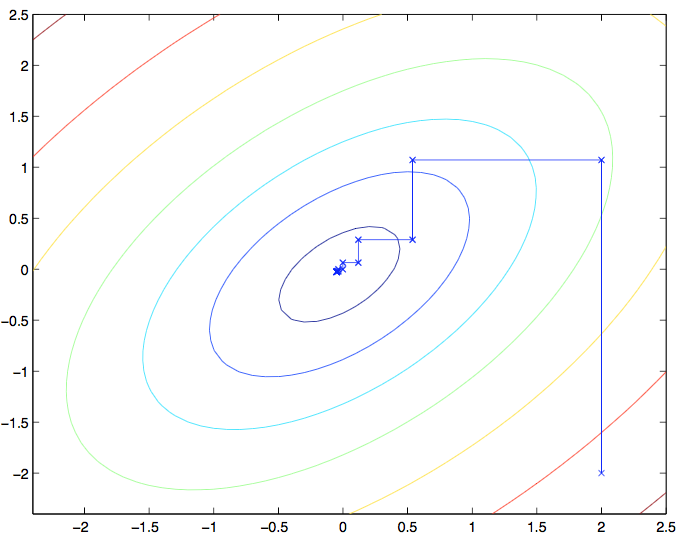
\includegraphics[scale=0.8]{./images/坐标上升}
		\caption{坐标上升示意图}
	\end{figure}
\end{enumerate}


\subsubsection{SMO}
在我们的SVM中,如果还是像前面的坐标上升算法那样固定住除$\alpha_j$以外的所有$\alpha$,那么,因为约束条件的存在,$\alpha_j$也被约束条件固定下来了,所以,我们就让两个$\alpha$可变,这就有了SMO。\\
详略,暂时不想写,参考资料:\url{http://www.cnblogs.com/jerrylead/archive/2011/03/18/1988419.html}

		\subsection{SVM代码实现}
\subsubsection{Cost Function}
\begin{equation}\begin{aligned}
	J(\theta) = C\sum_{i=1}^m y^{(i)}cost_1(\theta^Tx^{(i)}) + (1-y^{(i)})cost_0(\theta^Tx^{(i)}) + \frac{1}{2}\sum_{j=1}^n\Theta_j^2
\end{aligned}\end{equation}
其中,$cost_1(\theta^Tx^{(i)})$对应$y=1$; $cost_0(\theta^Tx^{(i)})$对应$y=0$


\subsubsection{Gaussian Kernel}
\begin{equation}\begin{aligned}
	f_i = similarity(x, l^{(i)}) = exp(-\frac{\sum_{j=1}^n(x_j - l_j^{(i)})^2}{2\sigma^2})
\end{aligned}\end{equation}
\begin{enumerate}
	\item 当$x \approx l^{(i)}$时,$f_i=exp(-\frac{\approx 0^2}{2\sigma^2}) \approx 1$
	\item 当$x$远离$l^{(i)}$时,$f_i=exp(-\frac{inf^2}{2\sigma^2}) \approx 1$
	\item 3
\end{enumerate}


\subsubsection{SVM中,$C$与$\sigma^2$对欠拟合或过拟合的影响}
\begin{enumerate}
	\item C:C过大:低偏差,高方差;C过小:高偏差,第方差
	\item $\lambda^2$: 过大: 高偏差,低方差;过小: 低偏差,高方差
\end{enumerate}


\subsubsection{如何选项使用Logistic Regression还是 SVM}
\begin{enumerate}
	\item $n$很大时,使用Logistic Regression或无kernel(即linear kernel)的SVM
	\item $n$很小,$m$中等:使用Gaussian kernel的SVM
	\item $n$很小,$m$很大:增加特征,并使使用Logistic Regression或无kernel(即linear kernel)的SVM
	\item 神经网络可能更加适合,但是使用神经网络训练需要耗费的时间较长
\end{enumerate}



	\section{神经网络}
\subsection{神经网络--前向算法}

\subsubsection{各矩阵形式}
\begin{enumerate}
\item X
\begin{equation} \begin{aligned}
	X & = \left(\begin{matrix}
			(x^{(1)})^T \\ (x^{(2)})^T \\ (x^{(3)})^T \\ \vdots \\ (x^{(m)})^T \\
		\end{matrix}\right) \\
	& = \left( \begin{matrix}
			x_1^{(1)} & x_2^{(1)} & x_3^{(1)} & \dots & x_n^{(1)} \\
			x_1^{(2)} & x_2^{(2)} & x_3^{(2)} & \dots & x_n^{(2)} \\
			x_1^{(3)} & x_2^{(3)} & x_3^{(3)} & \dots & x_n^{(3)} \\
			\vdots    & \vdots    & \vdots    & \ddots & \vdots   \\
			x_1^{(m)} & x_2^{(m)} & x_3^{(m)} & \dots & x_n^{(m)} \\
			\end{matrix}\right) \\
	& = \left(\begin{matrix}
			x_1^{(1)} & x_2^{(1)} & x_3^{(1)} & \dots & x_n^{(1)} \\
			x_1^{(2)} & x_2^{(2)} & x_3^{(2)} & \dots & x_n^{(2)} \\
			x_1^{(3)} & x_2^{(3)} & x_3^{(3)} & \dots & x_n^{(3)} \\
			\vdots    & \vdots    & \vdots    & \ddots & \vdots   \\
			x_1^{(m)} & x_2^{(m)} & x_3^{(m)} & \dots & x_n^{(m)} \\
		\end{matrix}\right), \quad {\rm I\!R}^{(m,n)}
\end{aligned} \end{equation}

\item $a^{(1)}$
\begin{equation}
	a^{(1)} = X , \quad {\rm I\!R}^{(m,n)}
\end{equation}

\item $\Theta^{(1)}$
\begin{equation}
\Theta^{(1)} = 
	\left(\begin{matrix}
		\theta_{10}^{(1)} & \theta_{11}^{(1)} & \theta_{12}^{(1)} & \dots & \theta_{1,s_1}^{(1)} \\
		\theta_{20}^{(1)} & \theta_{21}^{(1)} & \theta_{22}^{(1)} & \dots & \theta_{2,s_1}^{(1)} \\
		\theta_{30}^{(1)} & \theta_{31}^{(1)} & \theta_{32}^{(1)} & \dots & \theta_{3,s_1}^{(1)} \\
		\vdots    & \vdots    & \vdots    & \ddots & \vdots   \\
		\theta_{s_{2}0}^{(1)} & \theta_{s_{2}1}^{(1)} & \theta_{s_{2}2}^{(1)} & \dots & \theta_{s_{2},s_{1}}^{(1)}
	\end{matrix}\right), \quad {\rm I\!R}^{(s_{2},s_1+1)=(s_{2},n+1)}
\end{equation}

\item $z^{(2)}$ \\
给$a^{(1)}$的每个数据均添加上$a_0 = 1$后与$\Theta^{(1)}$计算,得到$z^{(2)}
\footnote{从$a^{(1)}$得到$a^{(2)}$需要经过sigmoid()函数,后续的从$a^{(j)}$得到$a^{(j+1)}$均需要经过sigmoid()函数}
=(1, a^{(1)})(\Theta^{(1)})^T$
\begin{equation}\begin{aligned}
	z^{(2)} &= (1, a^{(1)}) (\Theta^{(1)})^T \Rightarrow (m,n+1) * (n+1,s_{2})
		\\ &= 
		  \left(\begin{matrix}
				1 & x_1^{(1)} & x_2^{(1)} & x_3^{(1)} & \dots & x_n^{(1)} \\
				1 & x_1^{(2)} & x_2^{(2)} & x_3^{(2)} & \dots & x_n^{(2)} \\
				1 & x_1^{(3)} & x_2^{(3)} & x_3^{(3)} & \dots & x_n^{(3)} \\
				\vdots        & \vdots    & \vdots    & \vdots    & \ddots & \vdots   \\
				1 & x_1^{(m)} & x_2^{(m)} & x_3^{(m)} & \dots & x_n^{(m)} \\
			\end{matrix}\right)
			\left(\begin{matrix}
				\theta_{10}^{(1)} & \theta_{11}^{(1)} & \theta_{12}^{(1)} & \dots & \theta_{1,n}^{(1)} \\
				\theta_{20}^{(1)} & \theta_{21}^{(1)} & \theta_{22}^{(1)} & \dots & \theta_{2,n}^{(1)} \\
				\theta_{30}^{(1)} & \theta_{31}^{(1)} & \theta_{32}^{(1)} & \dots & \theta_{3,n}^{(1)} \\
				\vdots    & \vdots    & \vdots    & \ddots & \vdots   \\
				\theta_{s_{2},0}^{(j)} & \theta_{s_{2},1}^{(j)} & \theta_{s_{2},2}^{(j)} & \dots & \theta_{s_{2},n}^{(1)}
			\end{matrix}\right)^T
		\\ &= 
		  \left(\begin{matrix}
				1 & x_1^{(1)} & x_2^{(1)} & x_3^{(1)} & \dots & x_n^{(1)} \\
				1 & x_1^{(2)} & x_2^{(2)} & x_3^{(2)} & \dots & x_n^{(2)} \\
				1 & x_1^{(3)} & x_2^{(3)} & x_3^{(3)} & \dots & x_n^{(3)} \\
				\vdots        & \vdots    & \vdots    & \vdots    & \ddots & \vdots   \\
				1 & x_1^{(m)} & x_2^{(m)} & x_3^{(m)} & \dots & x_n^{(m)} \\
			\end{matrix}\right)
			\left(\begin{matrix}
				\theta_{10}^{(1)} & \theta_{20}^{(1)} & \theta_{30}^{(1)} & \dots & \theta_{s_{2},0}^{(1)} \\
				\theta_{11}^{(1)} & \theta_{21}^{(1)} & \theta_{31}^{(1)} & \dots & \theta_{s_{2},1}^{(1)} \\
				\theta_{12}^{(1)} & \theta_{22}^{(1)} & \theta_{32}^{(1)} & \dots & \theta_{s_{2},2}^{(1)} \\
				\theta_{13}^{(1)} & \theta_{23}^{(1)} & \theta_{33}^{(1)} & \dots & \theta_{s_{2},3}^{(1)} \\
				\vdots    & \vdots    & \vdots    & \ddots & \vdots   \\
				\theta_{1,n}^{(1)} & \theta_{2,n}^{(1)} & \theta_{3,n}^{(1)} & \dots & \theta_{s_{2},n}^{(1)}
			\end{matrix}\right)
		\\ &=
			\left(\begin{matrix}
				z^{(2)(1)} \\ z^{(2)(2)} \\ z^{(2)(3)} \\ \vdots \\ z^{(2)(m)} 
			\end{matrix}\right)
		\\ &= 
			\left(\begin{matrix}
				z_1^{(2)(1)} & z_2^{(2)(1)} & z_3^{(2)(1)} & \dots & z_{s_2}^{(2)(1)} \\
				z_1^{(2)(2)} & z_2^{(2)(2)} & z_3^{(2)(2)} & \dots & z_{s_2}^{(2)(2)} \\
				z_1^{(2)(3)} & z_2^{(2)(3)} & z_3^{(2)(3)} & \dots & z_{s_2}^{(2)(3)} \\
				\vdots & \vdots & \vdots & \ddots & \vdots \\
				z_1^{(2)(m)} & z_2^{(2)(m)} & z_3^{(2)(m)} & \dots & z_{s_2}^{(2)(m)} \\
			\end{matrix}\right), \quad {\rm I\!R}^{(m,n+1) * (n+1, s_{2})=(m,s_2)}
\end{aligned}\end{equation}
\footnote{上式$z_{s_2}^{(2)(m)}$中,$(2)$表示第2层神经网络,$(m)$表示第m个训练集,$s_2$表示第2层神经网络的最后一个单元}


\item $a^{(2)}$
\begin{equation}
	a^{(2)}=g(z^{(2)}), \quad {\rm I\!R}^{(m,s_2)}
\end{equation}

\item 后续同理 \\
\begin{equation}\begin{aligned}
	\Theta^{(2)} &= 
		\left(\begin{matrix}
			\theta_{10}^{(2)} & \theta_{11}^{(2)} & \theta_{12}^{(2)} & \dots & \theta_{1,s_2}^{(2)} \\
			\theta_{20}^{(2)} & \theta_{21}^{(2)} & \theta_{22}^{(2)} & \dots & \theta_{2,s_2}^{(2)} \\
			\theta_{30}^{(2)} & \theta_{31}^{(2)} & \theta_{32}^{(2)} & \dots & \theta_{3,s_2}^{(2)} \\
			\vdots    & \vdots    & \vdots    & \ddots & \vdots   \\
			\theta_{s_{3}0}^{(2)} & \theta_{s_{3}1}^{(2)} & \theta_{s_{3}2}^{(2)} & \dots & \theta_{s_{3},s_{2}}^{(2)}
		\end{matrix}\right), \quad {\rm I\!R}^{(s_{3},s_2+1)}\\
	z^{(3)} &= (1, a^{(2)}) (\Theta^{(2)})^T, \quad {\rm I\!R}^{(m,s_2+1) * (s_2+1, s_3)=(m,s_3)} \\
	& \vdots \\
\end{aligned} \end{equation}

\item 一般式
\begin{equation}\begin{aligned}
	a^{(j)} &= g(z^{(j-1)}), \quad {\rm I\!R}^{(m,s_j)} \\
	\Theta^{(j)} &= 
		\left(\begin{matrix}
			\theta_{10}^{(j)} & \theta_{11}^{(j)} & \theta_{12}^{(j)} & \dots & \theta_{1,s_{j}}^{(j)} \\
			\theta_{20}^{(j)} & \theta_{21}^{(j)} & \theta_{22}^{(j)} & \dots & \theta_{2,s_{j}}^{(j)} \\
			\theta_{30}^{(j)} & \theta_{31}^{(j)} & \theta_{32}^{(j)} & \dots & \theta_{3,s_{j}}^{(j)} \\
			\vdots    & \vdots    & \vdots    & \ddots & \vdots   \\
			\theta_{s_{j+1}0}^{(j)} & \theta_{s_{j+1}1}^{(j)} & \theta_{s_{j+1}2}^{(j)} & \dots & \theta_{s_{j+1},s_{j}}^{(j)}
		\end{matrix}\right), \quad {\rm I\!R}^{(s_{j+1},s_{j}+1)}\\
	z^{(j+1)} &= (1, a^{(j)}) (\Theta^{(j)})^T \\
		% \\ &= 
		%   \left(\begin{matrix}
		% 		1 & x_1^{(1)} & x_2^{(1)} & x_3^{(1)} & \dots & x_n^{(1)} \\
		% 		1 & x_1^{(2)} & x_2^{(2)} & x_3^{(2)} & \dots & x_n^{(2)} \\
		% 		1 & x_1^{(3)} & x_2^{(3)} & x_3^{(3)} & \dots & x_n^{(3)} \\
		% 		\vdots        & \vdots    & \vdots    & \vdots    & \ddots & \vdots   \\
		% 		1 & x_1^{(m)} & x_2^{(m)} & x_3^{(m)} & \dots & x_n^{(m)} \\
		% 	\end{matrix}\right)
		% 	\left(\begin{matrix}
		% 		\theta_{10}^{(1)} & \theta_{11}^{(1)} & \theta_{12}^{(1)} & \dots & \theta_{1,n}^{(1)} \\
		% 		\theta_{20}^{(1)} & \theta_{21}^{(1)} & \theta_{22}^{(1)} & \dots & \theta_{2,n}^{(1)} \\
		% 		\theta_{30}^{(1)} & \theta_{31}^{(1)} & \theta_{32}^{(1)} & \dots & \theta_{3,n}^{(1)} \\
		% 		\vdots    & \vdots    & \vdots    & \ddots & \vdots   \\
		% 		\theta_{s_{2},0}^{(j)} & \theta_{s_{2},1}^{(j)} & \theta_{s_{2},2}^{(j)} & \dots & \theta_{s_{2},n}^{(1)}
		% 	\end{matrix}\right)^T
		\\ &= 
		  \left(\begin{matrix}
				1 & a_1^{(j)(1)} & a_2^{(j)(1)} & a_3^{(j)(1)} & \dots & a_{s_j}^{(j)(1)} \\
				1 & a_1^{(j)(2)} & a_2^{(j)(2)} & a_3^{(j)(2)} & \dots & a_{s_j}^{(j)(2)} \\
				1 & a_1^{(j)(3)} & a_2^{(j)(3)} & a_3^{(j)(3)} & \dots & a_{s_j}^{(j)(3)} \\
				\vdots        & \vdots    & \vdots    & \vdots    & \ddots & \vdots   \\
				1 & a_1^{(j)(m)} & a_2^{(j)(m)} & a_3^{(j)(m)} & \dots & a_{s_j}^{(j)(m)} \\
			\end{matrix}\right)
			\left(\begin{matrix}
				\theta_{10}^{(j)} & \theta_{20}^{(j)} & \theta_{30}^{(j)} & \dots & \theta_{s_{j+1},0}^{(j)} \\
				\theta_{11}^{(j)} & \theta_{21}^{(j)} & \theta_{31}^{(j)} & \dots & \theta_{s_{j+1},1}^{(j)} \\
				\theta_{12}^{(j)} & \theta_{22}^{(j)} & \theta_{32}^{(j)} & \dots & \theta_{s_{j+1},2}^{(j)} \\
				\theta_{13}^{(j)} & \theta_{23}^{(j)} & \theta_{33}^{(j)} & \dots & \theta_{s_{j+1},3}^{(j)} \\
				\vdots    & \vdots    & \vdots    & \ddots & \vdots   \\
				\theta_{1,s_j}^{(j)} & \theta_{2,s_j}^{(j)} & \theta_{3,s_j}^{(j)} & \dots & \theta_{s_{j+1},s_j}^{(j)}
			\end{matrix}\right)
		\\ &=
			\left(\begin{matrix}
				z^{(j+1)(1)} \\ z^{(j+1)(2)} \\ z^{(j+1)(3)} \\ \vdots \\ z^{(j+1)(m)} 
			\end{matrix}\right)
		\\ &= 
			\left(\begin{matrix}
				z_1^{(j+1)(1)} & z_2^{(j+1)(1)} & z_3^{(j+1)(1)} & \dots & z_{s_{j+1}}^{(j+1)(1)} \\
				z_1^{(j+1)(2)} & z_2^{(j+1)(2)} & z_3^{(j+1)(2)} & \dots & z_{s_{j+1}}^{(j+1)(2)} \\
				z_1^{(j+1)(3)} & z_2^{(j+1)(3)} & z_3^{(j+1)(3)} & \dots & z_{s_{j+1}}^{(j+1)(3)} \\
				\vdots & \vdots & \vdots & \ddots & \vdots \\
				z_1^{(j+1)(m)} & z_2^{(j+1)(m)} & z_3^{(j+1)(m)} & \dots & z_{s_{j+1}}^{(j+1)(m)} \\
			\end{matrix}\right)
		\\ &, \quad {\rm I\!R}^{(m,s_j+1) * (s_j+1, s_{j+1}) = (m,s_{j+1})} \\
	a^{(j+1)} &= g(z^{(j+1)}), \quad {\rm I\!R}^{(m,s_{j+1})}
\end{aligned}\end{equation}
\end{enumerate}

\subsubsection{y}
\begin{equation} \begin{aligned}
	y & = \left(\begin{matrix}
			y^{(1)} \\ y^{(2)} \\ y^{(3)} \\ \vdots \\ y^{(m)} \\
		\end{matrix}\right), \quad {\rm I\!R}^{m*1}
\end{aligned} \end{equation}

为进行矩阵运算,要将其转化为如下形式:\footnote{y所对应的值所在的索引位置值为1,其他位置均为0}
\begin{equation}\begin{aligned}
	Y &= \left(\begin{matrix}
	        0 & 0 & 0 & \dots & 0 & 1 \\
	        0 & 1 & 0 & \dots & 0 & 0 \\
	        0 & 0 & 1 & \dots & 0 & 0 \\
	        \vdots & \vdots & \vdots & \vdots & \ddots & \vdots \\
	        1 & 0 & 0 & \dots & 0 & 0 \\
		\end{matrix}\right), \quad {\rm I\!R}^{m,s_L}
\end{aligned}\end{equation}\footnote{上式$m*s_L$中的$s_L$表示共有$s_L$个分类器,$s_L$表示的是输出层的unit数}

		\subsection{神经网络--前向算法示意图}
\begin{tikzpicture}
\tikzset{
	a/.style={circle, draw=black}
}

% x
% \node[a] (x_0) at(0,10) {$x_0=+1$};
\node[a] (x_1) at(0,8) {$x_1$};
\node[a] (x_2) at(0,6) {$x_2$};
\node[a] (x_3) at(0,4) {$x_3$};
\filldraw (0,3) circle (.06);
\filldraw (0,2) circle (.06);
\filldraw (0,1) circle (.06);
\node[a] (x_n) at(0,0) {$x_n$};

% X与a的分隔线
\draw [dashed] (1,-1) -- (1,9);

% a^{(1)}
\node[a] (a_10) at(2,10)   {$+1$};
\node[a] (a_11) at(2,8)   {$a_1^{(1)}$};
\node[a] (a_12) at(2,6) {$a_2^{(1)}$};
\node[a] (a_13) at(2,4)   {$a_3^{(1)}$};
\filldraw (2,3) circle (.06);
\filldraw (2,2) circle (.06);
\filldraw (2,1) circle (.06);
\node[a] (a_1s1) at(2,0) {$a_{s_1}^{(1)}$};

% a^{(2)}
\node[a] (a_20) at(6,9.5) {$+1$};
\node[a] (a_21) at(6,8.0) {$a_1^{(2)}$};
\node[a] (a_22) at(6,6.5) {$a_2^{(2)}$};
\node[a] (a_23) at(6,5.0) {$a_3^{(2)}$};
\node[a] (a_24) at(6,3.5) {$a_4^{(2)}$};
\filldraw (6,2.4) circle (.06);
\filldraw (6,1.8) circle (.06);
\filldraw (6,1.2) circle (.06);
\node[a] (a_2s2) at(6,0) {$a_{s_2}^{(2)}$};

% a^{(3)}
\node[a] (a_30) at(10,9.5) {$+1$};
\node[a] (a_31) at(10,8.0) {$a_1^{(3)}$};
\node[a] (a_32) at(10,6.5) {$a_2^{(3)}$};
\node[a] (a_33) at(10,5.0) {$a_3^{(3)}$};
\node[a] (a_34) at(10,3.5) {$a_4^{(3)}$};
\filldraw (10,2.4) circle (.06);
\filldraw (10,1.8) circle (.06);
\filldraw (10,1.2) circle (.06);
\node[a] (a_3s3) at(10,0) {$a_{s_3}^{(3)}$};

% 中间部分
\filldraw (12,0) circle (.06);
\filldraw (12,2) circle (.06);
\filldraw (12,4) circle (.06);
\filldraw (12,6) circle (.06);
\filldraw (12,8) circle (.06);

% a^{(n)}

\node[a] (a_L1) at(14,7.5) {$a_1^{(L)}$};
\node[a] (a_L2) at(14,6)   {$a_2^{(L)}$};
\node[a] (a_L3) at(14,4.5) {$a_3^{(L)}$};
\node[a] (a_L4) at(14,3)   {$a_4^{(L)}$};
\filldraw (14,2.0) circle (.06);
\filldraw (14,1.5) circle (.06);
\filldraw (14,1.0) circle (.06);
\node[a] (a_Lsl) at(14,0) {$a_{s_l}^{(L)}$};


% 前向算法图例--仅连线:a1 -- a_21
% \draw[->] (a_10) -- (a_21);
\draw[->] (a_11) -- (a_21);
\draw[->] (a_12) -- (a_21);
\draw[->] (a_13) -- (a_21);
% \draw[->] (a_1s1) -- (a_21);

% 前向算法图例--有标注:a1 -- a_21
\path (a_10) edge[->] node[auto] {$\theta_{10}^{(1)}$} (a_21);
% \path (a_11) edge[->] node[auto] {$\theta_{11}^{(1)}$} (a_21);
% \path (a_12) edge[->] node[auto] {$\theta_{12}^{(1)}$} (a_21);
% \path (a_13) edge[->] node[auto] {$\theta_{13}^{(1)}$} (a_21);
\path (a_1s1) edge[->] node[auto] {$\theta_{1s1}^{(1)}$} (a_21);


% 前向算法--仅连线: a2 --> a34
% \draw[->] (a_20) -- (a_34);
\draw[->] (a_21) -- (a_34);
\draw[->] (a_22) -- (a_34);
\draw[->] (a_23) -- (a_34);
\draw[->] (a_24) -- (a_34);
% \draw[->] (a_2s2) -- (a_34);

% 前后算法图例--有标注:a2 -- a34
\path (a_20) edge[->] node[auto] {$\theta_{40}^{(2)}$} (a_34);
% \path (a_21) edge[->] node[auto] {$\theta_{41}^{(2)}$} (a_34);
% \path (a_22) edge[->] node[auto] {$\theta_{42}^{(2)}$} (a_34);
% \path (a_23) edge[->] node[auto] {$\theta_{43}^{(2)}$} (a_34);
% \path (a_24) edge[->] node[auto] {$\theta_{44}^{(2)}$} (a_34);
\path (a_2s2) edge[->] node[auto] {$\theta_{4s2}^{(2)}$} (a_34);


% 下方的标志
\node at (4, 11) {\color{red}{$\Theta^{(1)}$}};
\node at (8, 11) {\color{red}{$\Theta^{(2)}$}};

\end{tikzpicture}


\begin{equation}
	a^{(j)} = g(z^{(j-1)}) \Rightarrow {(m,s_j)}
\end{equation}

\begin{equation}
	\Theta^{(j)} = 
		\left(\begin{matrix}
			\theta_{10}^{(j)} & \theta_{11}^{(j)} & \theta_{12}^{(j)} & \dots & \theta_{1,s_{j}}^{(j)} \\
			\theta_{20}^{(j)} & \theta_{21}^{(j)} & \theta_{22}^{(j)} & \dots & \theta_{2,s_{j}}^{(j)} \\
			\theta_{30}^{(j)} & \theta_{31}^{(j)} & \theta_{32}^{(j)} & \dots & \theta_{3,s_{j}}^{(j)} \\
			\vdots    & \vdots    & \vdots    & \ddots & \vdots   \\
			\theta_{s_{j+1}0}^{(j)} & \theta_{s_{j+1}1}^{(j)} & \theta_{s_{j+1}2}^{(j)} & \dots & \theta_{s_{j+1},s_{j}}^{(j)}
		\end{matrix}\right) \Rightarrow {(s_{j+1},s_{j}+1)}
\end{equation}

\begin{equation}\begin{aligned}
	z^{(j+1)} &= (1, a^{(j)}) (\Theta^{(j)})^T \\
		\\ &= 
			\left(\begin{matrix}
				z_1^{(j+1)(1)} & z_2^{(j+1)(1)} & z_3^{(j+1)(1)} & \dots & z_{s_{j+1}}^{(j+1)(1)} \\
				z_1^{(j+1)(2)} & z_2^{(j+1)(2)} & z_3^{(j+1)(2)} & \dots & z_{s_{j+1}}^{(j+1)(2)} \\
				z_1^{(j+1)(3)} & z_2^{(j+1)(3)} & z_3^{(j+1)(3)} & \dots & z_{s_{j+1}}^{(j+1)(3)} \\
				\vdots & \vdots & \vdots & \ddots & \vdots \\
				z_1^{(j+1)(m)} & z_2^{(j+1)(m)} & z_3^{(j+1)(m)} & \dots & z_{s_{j+1}}^{(j+1)(m)} \\
			\end{matrix}\right)
\end{aligned}\end{equation}

\begin{equation}
	a^{(j+1)} = g(z^{(j)})  \Rightarrow {(m,s_{j+1})} 
\end{equation}


\begin{equation} \begin{aligned}
	y & = \left(\begin{matrix}
			y^{(1)} \\ y^{(2)} \\ y^{(3)} \\ \vdots \\ y^{(m)} \\
		\end{matrix}\right)_{m*1}
\end{aligned} \end{equation}

		\subsection{神经网络--后向算法}

\subsubsection{输出层结果:$a^L$}
\begin{equation}
	a^L = 
		\left(\begin{matrix}
			a_1^{(L)(1)} & a_2^{(L)(1)} & a_3^{(L)(1)} & \dots & a_{s_L}^{(L)(1)} \\
			a_1^{(L)(2)} & a_2^{(L)(2)} & a_3^{(L)(2)} & \dots & a_{s_L}^{(L)(2)} \\
			a_1^{(L)(3)} & a_2^{(L)(3)} & a_3^{(L)(3)} & \dots & a_{s_L}^{(L)(3)} \\
			\vdots & \vdots & \vdots & \ddots & \vdots \\
			a_1^{(L)(m)} & a_2^{(L)(m)} & a_3^{(L)(m)} & \dots & a_{s_L}^{(L)(m)} \\
		\end{matrix}\right), \quad {\rm I\!R}^{m,s_L}
\end{equation}

\subsubsection{格式化后的Y}
\begin{equation}\begin{aligned}
	Y &= \left(\begin{matrix}
	        0 & 0 & 0 & \dots & 0 & 1 \\
	        0 & 1 & 0 & \dots & 0 & 0 \\
	        0 & 0 & 1 & \dots & 0 & 0 \\
	        \vdots & \vdots & \vdots & \vdots & \ddots & \vdots \\
	        1 & 0 & 0 & \dots & 0 & 0 \\
		\end{matrix}\right), \quad {\rm I\!R}^{m,s_L}
\end{aligned}\end{equation}

\subsubsection{$\delta^{L}$}
\begin{equation}\begin{aligned}
	\delta^{L} &= a^{L} - y \\
		&= \left(\begin{matrix}
			a_1^{(L)} \\ a_2^{(L)} \\ a_3^{(L)} \\ \vdots \\ a_{s_L}^{(L)}
		\end{matrix}\right) - 
		\left(\begin{matrix}
	        1 \\ 0 \\ 0 \\ \vdots \\ 0 \\ 0 
		\end{matrix}\right)
\end{aligned}\end{equation}
\begin{itemize}
	\item 此时,$\delta^{L}, a^{L}, y$表示的是均向量(不是矩阵)
\end{itemize}

% \begin{equation}\begin{aligned}
% 	\Delta^{L} &= a^{L} - Y \\
% 	&= 	
% 		\left(\begin{matrix}
% 			a_1^{(L)(1)} & a_2^{(L)(1)} & a_3^{(L)(1)} & \dots & a_{s_L}^{(L)(1)} \\
% 			a_1^{(L)(2)} & a_2^{(L)(2)} & a_3^{(L)(2)} & \dots & a_{s_L}^{(L)(2)} \\
% 			a_1^{(L)(3)} & a_2^{(L)(3)} & a_3^{(L)(3)} & \dots & a_{s_L}^{(L)(3)} \\
% 			\vdots & \vdots & \vdots & \ddots & \vdots \\
% 			a_1^{(L)(m)} & a_2^{(L)(m)} & a_3^{(L)(m)} & \dots & a_{s_L}^{(L)(m)} \\
% 		\end{matrix}\right) - 
% 		 \left(\begin{matrix}
% 	        0 & 0 & 0 & \dots & 0 & 1 \\
% 	        0 & 1 & 0 & \dots & 0 & 0 \\
% 	        0 & 0 & 1 & \dots & 0 & 0 \\
% 	        \vdots & \vdots & \vdots & \vdots & \ddots & \vdots \\
% 	        1 & 0 & 0 & \dots & 0 & 0 \\
% 		\end{matrix}\right)_{m,s_L}
% \end{aligned}\end{equation}
% \begin{itemize}
% 	\item 此时,$\Delta^{L}, a^{L}, Y$表示的是均是矩阵
% 	\item {\color{red}{从教程看,似乎不用这样算,都用迭代的方式,这大概也是$\delta^{l}$ 与 $\Delta^{l}$表示的意义不一样的来源}}
% \end{itemize}

\subsubsection{$\delta^{L-1}$}
\begin{equation}\begin{aligned}
	\delta^{L-1} &= (\Theta^{(L-1)})^T \delta^{L} .* g^{'}(z^{L-1}) \\
	&= (\Theta^{(L-1)})^T \delta^{L} .* g(z^{L-1}) .* (1-g(z^{L-1}))
\end{aligned}\end{equation}
\begin{enumerate}
	\item 其中,式$g^{'}(z) = g(z)(1-g(z))$,此为sigmoid()函数的特性
	\item 此时,$z^{L-1}$表示的是一个向量(不是矩阵)
	\item 此时不需要舍弃$\delta_0^{L}$,因为根本就没有
\end{enumerate}

% \begin{equation}\begin{aligned}
% 	\Delta^{L-1} &= (\Theta^{(L-1)})^T \Delta^{L} .* g^{'}(z^{L-1}) \\
% 	&= (\Theta^{(L-1)})^T \Delta^{L} .* g(z^{L-1}) .* (1-g(z^{L-1}))
% \end{aligned}\end{equation}
% \begin{enumerate}
% 	\item 此时,$z^{L-1}$表示的是矩阵
% 	\item 与上述的$\delta^{L-1}$相比,此式批量计算的训练集中的所有数据
% 	\item {\color{red}{从教程看,似乎不用这样算,都用迭代的方式,这大概也是$\delta^{l}$ 与 $\Delta^{l}$表示的意义不一样的来源}}
% \end{enumerate}


\subsubsection{$\delta^{l}$($2<=l<=L-2$)}
\begin{equation}\begin{aligned}
	\delta^{l} &= (\Theta^{(l)})^T [\delta^{l+1}(2:end)] .* g^{'}(z^{l}) \\
	&= (\Theta^{(l)})^T [\delta^{l+1}(2:end)] .* g(z^{l}) .* (1-g(z^{l}))
\end{aligned}\end{equation}
\begin{enumerate}
	\item 因$a^{(1)}$直接从X得到,不会有误差,故无$\delta^{(1)}$
	\item (2:end)表示舍弃第一个数据$\delta_0^{s_{L-1}}$(Matlab索引从1开始)
	\item 对比于从$a^{l}$到$a^{l+1}$要添加一个$a_0^{l}=1$;从$\delta^{l+1}$到$\delta^{l}$要舍弃一个$\delta_0^{l+1}$
	\item 同样地,此时$z^{l}$表示的是一个向量(不是矩阵)
\end{enumerate}

\subsubsection{$\Delta^{l}$(用迭代的方式计算)}
\begin{enumerate}
	\item 数值计算方式
	\begin{equation}\begin{aligned}
		\Delta_{ij}^{(l)} := \Delta_{ij}^{(l)} + a_j^{(l)} \delta_i^{(l+1)}
	\end{aligned}\end{equation}
	\item 矩阵计算方式
	\begin{equation}\begin{aligned}
		\Delta^{(l)} := \Delta^{(l)} + \delta^{(l+1)} (a^{(l)})^T
	\end{aligned}\end{equation}
\end{enumerate}

\subsubsection{$D_{ij}^{(l)}$}
\begin{enumerate}
	\item $j=0$时
	\begin{equation}
		D_{ij}^{(l)} := \frac{1}{m}\Delta_{ij}^{(l)}
	\end{equation}
	\item $j \neq 0$时
		\begin{equation}
		D_{ij}^{(l)} := \frac{1}{m}(\Delta_{ij}^{(l)} + \Theta_{ij}^{(l)})
	\end{equation}
\end{enumerate}

\subsubsection{$\frac{\partial{J(\Theta)}}{\partial{\Theta_{ij}^{(l)}}}$}
\begin{equation}
	\frac{\partial{J(\Theta)}}{\partial{\Theta_{ij}^{(l)}}} = D_{ij}^{(l)}
\end{equation}

\subsubsection{$\delta^{l}$ 与 $\Delta^{l}$的区别与联系}














		\subsection{神经网络--后向算法示意图}
\begin{tikzpicture}
\tikzset{
	a/.style={circle, draw=black}
}

% x
% \node[a] (x_0) at(0,10) {$x_0=+1$};
\node[a] (x_1) at(0,8) {$x_1$};
\node[a] (x_2) at(0,6) {$x_2$};
\node[a] (x_3) at(0,4) {$x_3$};
\filldraw (0,3) circle (.06);
\filldraw (0,2) circle (.06);
\filldraw (0,1) circle (.06);
\node[a] (x_n) at(0,0) {$x_n$};

% X与a的分隔线
\draw [dashed] (1,-1) -- (1,9);

% \delta^{(1)}
\node[a] (a_10) at(2,10)   {0};
\node[a] (a_11) at(2,8)   {0};
\node[a] (a_12) at(2,6) {0};
\node[a] (a_13) at(2,4)   {0};
\filldraw (2,3) circle (.06);
\filldraw (2,2) circle (.06);
\filldraw (2,1) circle (.06);
\node[a] (a_1s1) at(2,0) {0};

% \delta^{(2)}
\node[a] (a_20) at(6,9.5) {$\delta_0^{(2)}$};
\node[a] (a_21) at(6,8.0) {$\delta_1^{(2)}$};
\node[a] (a_22) at(6,6.5) {$\delta_2^{(2)}$};
\node[a] (a_23) at(6,5.0) {$\delta_3^{(2)}$};
\node[a] (a_24) at(6,3.5) {$\delta_4^{(2)}$};
\filldraw (6,2.4) circle (.06);
\filldraw (6,1.8) circle (.06);
\filldraw (6,1.2) circle (.06);
\node[a] (a_2s2) at(6,0) {$\delta_{s_2}^{(2)}$};

% \delta^{(3)}
\node[a] (a_30) at(10,9.5) {$\delta_0^{(3)}$};
\node[a] (a_31) at(10,8.0) {$\delta_1^{(3)}$};
\node[a] (a_32) at(10,6.5) {$\delta_2^{(3)}$};
\node[a] (a_33) at(10,5.0) {$\delta_3^{(3)}$};
\node[a] (a_34) at(10,3.5) {$\delta_4^{(3)}$};
\filldraw (10,2.4) circle (.06);
\filldraw (10,1.8) circle (.06);
\filldraw (10,1.2) circle (.06);
\node[a] (a_3s3) at(10,0) {$\delta_{s_3}^{(3)}$};

% 中间部分
\filldraw (12,0) circle (.06);
\filldraw (12,2) circle (.06);
\filldraw (12,4) circle (.06);
\filldraw (12,6) circle (.06);
\filldraw (12,8) circle (.06);

% \delta^{(n)}

\node[a] (a_L1) at(14,7.5) {$\delta_1^{(L)}$};
\node[a] (a_L2) at(14,6)   {$\delta_2^{(L)}$};
\node[a] (a_L3) at(14,4.5) {$\delta_3^{(L)}$};
\node[a] (a_L4) at(14,3)   {$\delta_4^{(L)}$};
\filldraw (14,2.0) circle (.06);
\filldraw (14,1.5) circle (.06);
\filldraw (14,1.0) circle (.06);
\node[a] (a_Lsl) at(14,0) {$\delta_{s_l}^{(L)}$};


% % 后向算法图例--仅连线:\delta21 -- \delta_1
% \draw[->] (a_21) -- (a_10);
% \draw[->] (a_21) -- (a_11);
% \draw[->] (a_21) -- (a_12);
% \draw[->] (a_21) -- (a_13);
% \draw[->] (a_21) -- (a_1s1);
% % 后向算法图例--仅连线:\delta22 -- \delta_1
% \draw[->] (a_22) -- (a_10);
% \draw[->] (a_22) -- (a_11);
% \draw[->] (a_22) -- (a_12);
% \draw[->] (a_22) -- (a_13);
% \draw[->] (a_22) -- (a_1s1);
% % 后向算法图例--仅连线:\delta23 -- \delta_1
% \draw[->] (a_23) -- (a_10);
% \draw[->] (a_23) -- (a_11);
% \draw[->] (a_23) -- (a_12);
% \draw[->] (a_23) -- (a_13);
% \draw[->] (a_23) -- (a_1s1);
% % 后向算法图例--仅连线:\delta24 -- \delta_1
% \draw[->] (a_24) -- (a_10);
% \draw[->] (a_24) -- (a_11);
% \draw[->] (a_24) -- (a_12);
% \draw[->] (a_24) -- (a_13);
% \draw[->] (a_24) -- (a_1s1);
% % 后向算法图例--仅连线:\delta2s2 -- \delta_1
% \draw[->] (a_2s2) -- (a_10);
% \draw[->] (a_2s2) -- (a_11);
% \draw[->] (a_2s2) -- (a_12);
% \draw[->] (a_2s2) -- (a_13);
% \draw[->] (a_2s2) -- (a_1s1);


% 后向算法--仅连线: \delta31 --> \delta2
\draw[->] (a_31) -- (a_20);
\draw[->] (a_31) -- (a_21);
\draw[->] (a_31) -- (a_22);
\draw[->] (a_31) -- (a_23);
\draw[->] (a_31) -- (a_24);
\draw[->] (a_31) -- (a_2s2);
% 后向算法--仅连线: \delta32 --> \delta2
\draw[->] (a_32) -- (a_20);
\draw[->] (a_32) -- (a_21);
\draw[->] (a_32) -- (a_22);
\draw[->] (a_32) -- (a_23);
\draw[->] (a_32) -- (a_24);
\draw[->] (a_32) -- (a_2s2);
% 后向算法--仅连线: \delta33 --> \delta2
\draw[->] (a_33) -- (a_20);
\draw[->] (a_33) -- (a_21);
\draw[->] (a_33) -- (a_22);
\draw[->] (a_33) -- (a_23);
\draw[->] (a_33) -- (a_24);
\draw[->] (a_33) -- (a_2s2);
% 后向算法--仅连线: \delta34 --> \delta2
\draw[->] (a_34) -- (a_20);
\draw[->] (a_34) -- (a_21);
\draw[->] (a_34) -- (a_22);
\draw[->] (a_34) -- (a_23);
\draw[->] (a_34) -- (a_24);
\draw[->] (a_34) -- (a_2s2);
% 后向算法--仅连线: \delta3s3 --> \delta2
\draw[->] (a_3s3) -- (a_20);
\draw[->] (a_3s3) -- (a_21);
\draw[->] (a_3s3) -- (a_22);
\draw[->] (a_3s3) -- (a_23);
\draw[->] (a_3s3) -- (a_24);
\draw[->] (a_3s3) -- (a_2s2);


% 标志
\node at (4, 11) {$\Theta^{(1)}$};
\node at (8, 11) {$\Theta^{(2)}$};
\node at (2, -1) {\color{red}{无$\delta^{(1)}$}};
\node at (6, -1) {\color{red}{$\delta^{(2)}$}};
\node at (10, -1) {\color{red}{$\delta^{(3)}$}};


% \node at (4, -2) {\color{red}{$\delta^{(1)}=(\Theta^{(1)})^T [\delta^{2}(2:end)] .* g(z^{1}) .* (1-g(z^{1}))$}};
% \node at (8, -3) {\color{red}{$\delta^{(l)}=(\Theta^{(l)})^T [\delta^{l+1}(2:end)] .* g(z^{l}) .* (1-g(z^{l}))$}};


\end{tikzpicture}



\[\begin{cases}
	\delta^{L} &= a^{L} - y ,\quad l=L \\
	\delta^{L-1} &= (\Theta^{(L-1)})^T \delta^{L} .* g^{'}(z^{L-1}) \\
		&= (\Theta^{(L-1)})^T \delta^{L} .* g(z^{L-1}) .* (1-g(z^{L-1})),\quad l=L-1 \\
		\delta^{l} &= (\Theta^{(l)})^T [\delta^{l+1}(2:end)] .* g^{'}(z^{l}) \\
	&= (\Theta^{(l)})^T [\delta^{l+1}(2:end)] .* g(z^{l}) .* (1-g(z^{l})) ,\quad 2<=l<=L-2 \\
	% 无 a^{(1)}, \quad l=1
\end{cases}\] \\
无 $\delta^{(1)}$

\begin{equation}\begin{aligned}
		\Delta^{(l)} := \Delta^{(l)} + \delta^{(l+1)} (a^{(l)})^T
	\end{aligned}\end{equation}

\[ D_{ij}^{(l)} = \begin{cases}
	\frac{1}{m}\Delta_{ij}^{(l)} ,\quad j=0 \\
	\frac{1}{m}(\Delta_{ij}^{(l)} + \Theta_{ij}^{(l)}), \quad j \neq 0
\end{cases}\]

\begin{equation*}
	\frac{\partial{J(\Theta)}}{\partial{\Theta_{ij}^{(l)}}} = D_{ij}^{(l)}
\end{equation*}






	\section{经验风险最小化}

\subsection{偏差\&方差}
\begin{enumerate}
	\item 高偏差(Bias)对应欠拟合
	\item 高方差(Variance)对应过拟合
\end{enumerate}

\subsection{经验风险最小化(ERM)}
\begin{enumerate}
	\item 定义数据集:
	\begin{align}
		S = \{x^{(i)}, y^{(i)}\}, \quad 1 \leq i \leq m
	\end{align}
	其中,$x^{(i)}, y^{(i)}$独立同分布(IID),$y \in \{0, 1\}$
	\item 分类模型为:
	\begin{align}
		h_{\theta}(x) &= g(\theta^Tx) \\
		\text{其中:}
		g(z) &= 1\{z\geq 0\}, \quad g \in \{0, 1\}
	\end{align}
	所以,$h_{\theta}(x)$只会是$0$或$1$
	\item 定义训练误差为:
	\begin{align}
		\hat{\varepsilon}(h_{\theta}) = \hat{\varepsilon_S}(h_{\theta}) = \frac{1}{m}\sum_{i=1}^{m}1\{h_{\theta}(x^{(i)}) \neq y^{(i)}\}
	\end{align}
	\item 经验误差最小化为:
	\begin{align}
		\hat{\theta} = \arg_{\theta}\min{\hat{\varepsilon_S}(h_{\theta})}
	\end{align}
	即选择使训练误差最小的参数$\theta$。\\
	对于ERM来说,因为他是非凸的,用一般算法不好优化。
	\item 我们再定义另一种等价的ERM,首先假设模型集合:
	\begin{align}
		\mathcal{H} = \{h_{\theta}: \theta \in R^{n\times 1}\}
	\end{align}
	其中,$h_{\theta}$为分类模型,输出为$0$或$1$。
	\item 其训练误差为:
	\begin{align}
		\hat{\varepsilon}(h) = \frac{1}{m}\sum_{i=1}^{m}1\{h(x^{(i)}) \neq y^{(i)}\}
	\end{align}
	\item 那么,ERM定义为:
	\begin{align}
		\hat{h} = \arg_{h \in \mathcal{H}} \min{\hat{\varepsilon}(h)}
	\end{align}
	\item 泛化能力定义为:
	\begin{align}
		\varepsilon(h) = P_{x,y \sim D} (h(x) \neq y)
	\end{align}
	接下来的任务是证明最优化ERM能带来较小的泛化误差,为此,我们先引入两个引理。
\end{enumerate}


\subsection{联合界 \& Hoeffding不等式}
\subsubsection{联合界定理}
\begin{enumerate}
	\item 令$A_1, A_2, \dots, A_k$是$k$个任意事件(即不要求独立,也不要求同分布,也没有其他要求),那么:
	\begin{align}
		P(A_1 \cup A_2 \cup \dots \cup A_k) \leq P(A_1) + P(A_2) + \dots + P(A_k)
	\end{align}
	此定理可画图证明,不赘述
\end{enumerate}

\subsubsection{Hoeffding不等式定理}
\begin{enumerate}
	\item 令$Z_1, Z-2, \dots, Z_m$为$m$个独立同分布(IID)变量,他们都服从Bernoulli分布,即:
	\begin{align}
		P(Z_i = 1) &= \varphi \\
		P(Z_i = 0) &= 1 - \varphi
	\end{align}
	我们使用这$m$个数据来估计$\varphi$,得:
	\begin{align}
		\hat{\varphi} = \frac{1}{m}\sum_{i=1}^{m}Z_i
	\end{align}
	那么,Hoeffding不等式即为:对于任意固定的数$\gamma > 0$,存在:
	\begin{align}
		P(|\hat{\varphi} - \varphi| > \gamma) < 2e^{-2\gamma^2 m}
	\end{align}
	这个定理的意义在于,当样本数目$m$增大时,我们对参数的估计将越来越接近真实值。
\end{enumerate}


\subsection{一致收敛定理}
\begin{enumerate}
	\item 定义模型集合为:
	\begin{align}
		\mathcal{H} = \{h_1, h_2, \dots, h_k\}
	\end{align}
	\item 一致收敛定理为:\\
	\begin{align}
		P(\forall h_i \in \mathcal{H}, |\varepsilon(h_i)-\hat{\varepsilon(h_i)}|>\gamma) \geq 1- 2ke^{-2\gamma^2 m}
	\end{align}
	该式即为一致收敛定理,它的意义在于,至少有$1- 2ke^{-2\gamma^2 m}$的概率使得:对模型集合中的所有假设,其泛华误差都在训练误差的$\gamma$范围内。
\end{enumerate}



\subsection{一致收敛的推论}
在一致收敛中,三个参数$m, \gamma$,以及概率$P$是相互关联的,我们可以通过固定其中的2个来推出第三个。
\begin{enumerate}
	\item $P(m, \gamma)$上面已经给出,其余2个如下,证明过程略
	\item  $m$ 与$\gamma, P$的关系
	\begin{align}
		m \geq \frac{1}{2\gamma^2}\log\frac{2k}{\sigma}
	\end{align}
	此式说明了一个算法或模型要达到一个确定的性能时,需要的样本数目。也称为算法的样本复杂度。
	\item $\gamma$与$m, P$的关系
	\begin{align}
		\gamma = \sqrt{\frac{1}{2m}\log\frac{2k}{\sigma}}
	\end{align}

	\item 在一致收敛成立的情况下,我们通过ERM方法得到的假设$\hat{h}$的泛华能力如何?
	\begin{enumerate}
		\item 定义:
		\begin{align}
			h^* = \arg_{h\in\mathcal{H}}\min \varepsilon(h)
		\end{align}
		其中,$h^*$为泛华误差最小的假设
		\item 可以推导出:
		\begin{align}
			\varepsilon(\hat{h}) \leq \hat{\varepsilon}(\hat{h}) + \gamma \leq \hat{\varepsilon}(h^*) + \gamma \leq \varepsilon(h^*) + \gamma + \gamma
			= \varepsilon(h^*) + 2\gamma
		\end{align}


	\end{enumerate}
	{\color{red}{其余内容略,有用了再看。}}
\end{enumerate}

\subsection{说明}
\begin{enumerate}
	\item 本部分内容来源:斯坦福大学《机器学习公开课》第9课:\href{http://open.163.com/movie/2008/1/F/H/M6SGF6VB4_M6SGJV3FH.html}{经验风险最小化}
	\item 本笔记内容参考:本文参考以下笔记:\href{http://blog.csdn.net/stdcoutzyx/article/details/12110337}{课程笔记参考}
\end{enumerate}




	\section{VC维}
\subsection{打散}
\begin{enumerate}
	\item 打散的定义:设$\mathcal{F}$是一个决策函数候选集,即由在空间$R^n$上取值为$1$或$-1$的若干函数组成的集合;$Z_l=\{x_1, x_2, \dots, x_l\}$为$R^n$中的$l$个点组成的集合。如果对$Z_l$中各点$x_i$给予任意标号$y_i=1$或$y_i=-1$,并组成训练集:
	\begin{align}
		T = {(x_1, y_1), \dots, (x_l, y_l)}
	\end{align}
	$\mathcal{F}$中总存在一个函数$f$,它能完全正确地吧训练集分开,即满足:
	\begin{align}
		f(x_i) = y_i, \quad i = 1,\dots, l
	\end{align}
	则称$Z_l$能被$\mathcal{F}$打散。
\end{enumerate}


\subsection{VC维}
\begin{enumerate}
	\item 设$\mathcal{F}$是一个定义在空间$R^n$上,取值为$1$或$-1$的函数组成的决策函数候选集。定义$\mathcal{F}$的VC维为它能打散的$R^n$中的点的最大个数。
	\item 若存在$l$个点组成的集合$Z_l$能被$\mathcal{F}$打散,且任意$l+1$个点组成的集合$Z_{l+1}$都不能被$\mathcal{F}$打散,则$\mathcal{F}$的VC维就是$l$
	\item 若$\mathcal{F}$能打散任意多的点组成的集合,则说明这个$\mathcal{F}$的VC维为$\infty$
	\item 若$\mathcal{F}$的VC维较大,则这个$\mathcal{F}$较复杂;若较小,则较简单。

\end{enumerate}
{\color{red}{对VC维的理解还有待提高,待后续比较懂了再补充}}







































	\section{正则化与模式选择}
\subsection{模式选择}
在以下的内容中,我们定义$\mathcal{M} = \{M_1, M_2, \dots, M_d\}$为我们的Models Sets。

\subsubsection{交叉验证}
\begin{enumerate}
	\item Hold-Out Cross Validation(Simple Cross Validation)
	\begin{enumerate}
		\item 将数据集分为$70\%$的测试集与$30\%$的交叉验证集两份数据
		\item 使用$70\%$的测试集在Model Sets中对每个Model进行训练
		\item 用剩下的$30\%$对每个训练结果进行验证,选出经验误差$\hat{\varepsilon}_{S_{cv}}(h)$最小的作为我们要的Model,然后用所有的数据对选择的Model在进行训练
		\item $70\%$与$30\%$的比例可自行调整
		\item 使用此方法留给交叉验证集的数据太多了,于是后了下面的方式
	\end{enumerate}

	\item $k$-Fold Cross Validation
	\begin{enumerate}
		\item 将数据分成$k$份($k$的大小小于数据集大小$m$即可)
		\item 将第1份数据当做交叉训练集,用其余$k-1$份进行训练,并计算此时每个Model($M_i$)的误差$\hat{\varepsilon}_{S_1}(h_{i1})$
		\item 将第2份数据当做交叉训练集,用其余$k-1$份进行训练,并计算此时每个Model($M_i$)的误差$\hat{\varepsilon}_{S_2}(h_{i2})$
		\item 将第j份数据当做交叉训练集,用其余$k-1$份进行训练,并计算此时每个Model($M_i$)的误差$\hat{\varepsilon}_{S_j}(h_{ij})$
		\item 将第k份数据当做交叉训练集,用其余$k-1$份进行训练,并计算此时每个Model($M_i$)的误差$\hat{\varepsilon}_{S_k}(h_{ik})$
		\item 对每个Model用不同交叉验证集的到的误差取均值,选出误差最小的作为我们要的Model
		\item 使用$k$-Fold Cross Validation的缺点是计算量大,如$k=10$,我们就需要训练$10$次
		\item 特别地,若我们取$k=m$,则每次只留一个数据当做交叉验证集,我们将这种方式成为留一交叉验证(Leave-One-Out Cross Validation),一般只有在数据量很少时才会用此方法

	\end{enumerate}
\end{enumerate}


\subsection{特征选择}
当我们要训练的维度$n$非常大($n >> m$),但是并不一定所有的维度都对训练有利时,我们就希望能够选取部分的特征进行训练。

\subsubsection{向前搜索}
\begin{enumerate}
	\item 待添加
\end{enumerate}











		\subsection{贝叶斯统计与正则化}
在前面的逻辑回归讨论中,我们通过最大化似然函数来得到$\theta_{ML}$
\begin{align}
	\theta_{ML} = \arg \max_{\theta} \prod_{i=1}^{m}p(y^{(i)}|x^{(i)}; \theta)
\end{align}
在频率学派的观点中,$\theta$是一个参数,是一个定值(而不是随机的),只是我们暂时不知道它的大小是多少,我们的目的就是通过各种办法来预估$\theta$ \\
在贝叶斯学派的观点中,$\theta$被当做是随机变量(同样,他的值是未知的)。此时,我们称$p(\theta)$为$\theta$的先验分布。给定训练集$S=\{(x^{(i)}, y^{(i)})\}_{i=1}^{m}$,可得$\theta$的后验分布为:
\begin{align}
	p(\theta | S) &= \frac{p(X|\theta)p(\theta)}{p(S)} \\
	&= \frac{\left[\prod_{i=1}^{m}p(y^{(i)}|x^{(i)}, \theta) p(\theta)\right]}{\int_{\theta}\left[\prod_{i=1}^{m}p(y^{(i)}|x^{(i)}, \theta) p(\theta)\right]d\theta}
\end{align}
在上面的式子中,$p(y^{(i)}|x^{(i)}, \theta)$取决于你用什么算法,如用逻辑回归时,$p(y^{(i)}|x^{(i)}, \theta)=h_{\theta}(x^{(i)})^{y^{(i)}}\left[1-h_{\theta}(x^{(i)})\right]^{\left[1-y^{(i)}\right]}$\footnote{注意,此时,我们将$\theta$当做随机变量,因此,$\theta$与$x$间的分隔符号应为逗号,不是冒号了},其中,$h_{\theta}(x^{(i)})=\frac{1}{e^{-\theta^Tx^{(i)}}}$ \\
当我们要通过测试数据$x$进行预测时
\begin{align}
	p(y|x, S) = \int_{\theta}p(y|x, \theta)p(\theta|S)d\theta
\end{align}
期望:
\begin{align}
	E(y|x, S) = \int_{y}yp(y|x, S)dy
\end{align}
但是,因为在计算$p(\theta | S)$时需要耗费太多的性能,因此,我们并不会直接进行计算,而仅仅估计$p(\theta | S)$的值,称为最大化后验概率MAP(Maximum A Posteriori)
\begin{align}
	\theta_{MAP} = \arg \max_{\theta} \prod_{i=1}^{m}p(y^{(i)}|x^{(i)}, \theta)p(\theta)
\end{align}
有上式可以发现,最终的结果与最大化似然得到的一致。\\



























































		\subsection{正则化避免过拟合}
\subsubsection{线性回归}

\subsubsubsection{数值计算方式}
\begin{equation}
	J(\theta) = \frac{1}{2m}\sum_{i=1}^m [h_\theta(x^{(i)})-y^{(i)}]^2 + \lambda \frac{1}{2m} \sum_{j=1}^n\theta_j^2
\end{equation}

\begin{equation}\begin{aligned}
	\frac{\partial{J(\theta)}}{\partial{\theta_j}} &= \frac{1}{2m}\sum_{i=1}^m 2[h_\theta(x^{(i)}-y^{(i)})] \frac{\partial{h_\theta(x^{(i)})}}{\partial{\theta_j}} + \lambda \frac{1}{2m} 2  \theta_j \\
	    &= \frac{1}{m}\sum_{i=1}^m[h_\theta(x^{(i)})-y^{(i)}]x^{(i)} + \frac{\lambda}{m} \theta_j
\end{aligned}\end{equation}

\[\begin{cases}
	\theta_0 := \theta_0 - \alpha \frac{1}{m} \sum_{i=1}^m(h_\theta(x^{(i)}) - y^{(i)})x_0^{(i)}, \quad j=0 \\
	\theta_j := \theta_j - \alpha \frac{1}{m} \sum_{i=1}^m(h_\theta(x^{(i)}) - y^{(i)})x_j^{(i)} - \alpha\frac{\lambda}{m}\theta_j, \quad j \neq 0
\end{cases}\]



\subsubsubsection{矩阵计算方式}
\begin{equation}
	J(\theta) = \frac{1}{2m} \left[h_\theta(x) - y\right]^T \left[ h_\theta(x) - y\right] + \frac{\lambda}{2m} \sum_{j=1}^n\theta_j^2
\end{equation}

\begin{equation}
	\nabla J(\theta) = \frac{1}{2m} X^T \left[h_\theta(x) - y\right] + \frac{\lambda}{m} \theta_j
\end{equation}

% \[\begin{cases}
% 	\theta_0 := \theta_0 - \alpha \frac{1}{m} \sum_{i=1}^m(h_\theta(x^{(i)}) - y^{(i)})x_0^{(i)}, \quad j=0 \\
% 	\theta := \theta - \alpha \frac{1}{m} \sum_{i=1}^m(h_\theta(x^{(i)}) - y^{(i)})x^{(i)} + \alpha \frac{\lambda}{m}\theta, \quad j \neq 0
% \end{cases}\]

\[matlab\begin{cases}
	grad &= 1/m * X'*(h-y); , \quad\\
	grad(2:end) &= grad(2:end) + lambda/m * theta(2:end);
\end{cases}\]



\subsubsection{逻辑回归}

\subsubsubsection{数值计算方式}
\begin{equation}
	J(\theta) = \frac{1}{m}
	    \sum_{i=1}^m \left[ -y^{(i)}log{h_\theta(x^{(i)})} - (1-y^{(i)})log{(1-h_\theta(x^{(i)}))} \right]
		+ \lambda \frac{1}{2m} \sum_{j=1}^n\theta_j^2
\end{equation}

\[\begin{cases}
	\theta_0 := \theta_0 - \alpha \frac{1}{m} \sum_{i=1}^m(h_\theta(x^{(i)}) - y^{(i)})x_0^{(i)}, \quad j=0 \\
	\theta_j := \theta_j - \alpha \frac{1}{m} \sum_{i=1}^m(h_\theta(x^{(i)}) - y^{(i)})x_j^{(i)} - \alpha\frac{\lambda}{m}\theta_j, \quad j \neq 0
\end{cases}\]

\subsubsubsection{矩阵计算方式}
\begin{equation}
		J(\theta) = \frac{1}{m} \left[-y^T \log{h_\theta(x)} - (1-y^T) \log{(1-h_\theta(x)}\right] + \lambda \frac{1}{2m}\theta^T \theta
\end{equation}

% \[\begin{cases}
% 	\theta_0 := \theta_0 - \alpha \frac{1}{m} \sum_{i=1}^m(h_\theta(x^{(i)}) - y^{(i)})x_0^{(i)}, \quad j=0 \\
% 	\theta := \theta - \alpha \frac{1}{m} \sum_{i=1}^m(h_\theta(x^{(i)}) - y^{(i)})x^{(i)} + \alpha \frac{\lambda}{m}\theta, \quad j \neq 0
% \end{cases}\]

\[matlab\begin{cases}
	grad &= 1/m * X'*(h-y); , \quad\\
	grad(2:end) &= grad(2:end) + lambda/m * theta(2:end);
\end{cases}\]



\subsubsection{注意}
在实际计算$\theta$中,都是先计算没有Regularization的结果,再对(2:end)计算有Regularization的结果,再将其加到没有Regularization的结果中








	\section{k-Means}
k-Means算法是一个是一个无监督学习算法,此时,在我们的数据集中,仍旧有$x^{(i)} \in {\rm I\!R}^n$,但是没有$y^{(i)}$。

\subsection{k-Means聚类算法的计算步骤}
\begin{enumerate}
	\item 确定要聚类的数目$k$
	\item 随机初始化聚类中心$\mu_1, \mu_2, \dots, \mu_k$,可以任意选取$k$个数据点作为$k$个聚类中心的初始值,也可以使用其他的初始化方式
	\item 重复以下步骤,直到收敛
	\begin{enumerate}
		\item 计算每个数据点到每个聚类中心的距离平方值(当然,也可以使用其他计算方式,不过一般是用此方式。)
		\item 对每个数据点,取与其距离最近的聚类中心所属类别作为其新类别$c^{(i)}$
		\begin{align}
			c^{(i)} := \arg \min_j \|x^{(i)}-\mu_j\|^2
		\end{align}
		\item 对每个类别,使用当前类别中的的所有点,重新计算其聚类中心$\mu_j$
		\begin{align}
			\mu_j := \frac{\sum_{i=1}^{m}1\{c^{(i)}=j\}x^{(i)}}{\sum_{i=1}^{m}1\{c^{(i)}=j\}}
		\end{align}
		其中,$c^{(i)}$就是每个数据点在每次迭代中所属的新类别。
	\end{enumerate}
\end{enumerate}

\subsection{对k-Means算法的讨论}
\subsubsection{k-Means算法的收敛问题}
\begin{enumerate}
	\item Distortion Function
	\begin{align}
		J(c, \mu) = \sum_{i=1}^{m} \|x^{(i)} - \mu_{c^{(i)}}\|^2
	\end{align}
	如上式,$J(c, \mu)$描述的是每个数据$x^{(i)}$与聚类中心$\mu_{c^{(i)}}$的平方距离。
	\item 对于此式,我们可以用坐标下降的方法来对其进行优化:先固定$\mu$,改变$c$来对$J(c, \mu)$最小化;再固定$c$,改变$\mu$来对$J(c, \mu)$最小化。通过此方式,我们一定能让$J(c, \mu)$收敛。
	\item 因为$J(c, \mu)$并不是凸函数,所以通过坐标下降并不能保证收敛到全局最小值,而可能仅仅收敛到局部最小值。
	\item 为了避免我们的算法收敛到一个较差的局部最小值,我们可以多次用不同的方法初始化聚类中心,然后取其中效果最好的作为我们的优化结果。
\end{enumerate}














	\section{EM}
EM(Expectation-Maximization):期望最大化 \\

与前面的k-Means一样,假设我们的数据集为$\{x^{(1)}, x^{(2)}, \dots, x^{(m)}\}$,没有$y^{(i)}$,EM算法也是无监督学习算法。 \\

\begin{enumerate}
	\item 待优化模型:
	\begin{align}
		p(x^{(i)}, z^{(i)}) &= p(x^{(i)}|z^{(i)})p(z^{(i)})
	\end{align}
	其中,$z^{(i)}$服从多项式分布:
	\begin{align}
		z^{(i)} &\sim Multinomial(\phi), \quad \phi_j \geq 0 \\
		 \sum_{j=1}^{k}\phi_j &=1 \\ 
		 \phi_j &= p(z^{(i)}=j) \\
		 x^{(i)}|z^{(i)}=j &\sim \mathcal{N}(\mu_j, \sigma_j)
	\end{align}
\end{enumerate}



















	\section{调参技巧}

\subsection{Error Analysis}
\begin{enumerate}
	\item 0-1错分率 or 误分类率
	1. 将当前的数据分成2份,$70\%$作为训练集,$30\%$作为测试集\\
	2. 用新的训练集训练,用新的测试集检验效果\\
	3. 若$J_{train}(\theta)$很小,$J_{test}(\theta)$很大,则说明出现了过拟合
	\item 训练集 \& 交叉验证集 \& 测试集
	\item 过拟合、欠拟合的判断方法
	1. 欠拟合对应高偏差,表现为$J_{cv}(\theta) \approx J_{train}(\theta)$,且二者都很高 \\
	2. 过拟合对应高方差,表现为$J_{cv}(\theta) >> J_{train}(\theta)$,且$J_{train}(\theta)$很小 \\
	3. $J_{taain}(\theta)$对应训练集的学习能力;$J_{cv}(\theta)$对应训练结果对新样本的适应能力,适应能力越强,$J_{cv}(\theta)$越小 \\
	4. 在训练集和验证集(测试集)效果均不好,说明欠拟合;在训练集效果很好,但在说明欠拟合,但在验证集(测试集)效果不好,说明过拟合
\end{enumerate}

\subsection{Error Metrics for Skewed Classes}
\begin{enumerate}
	\item Skewed Classes
	那些两种(或多种)情况发生的概率相关较大的情况称为Skewed Classes。如买彩票中奖的概率与不中奖的概率
	\item True vs. False \& Positive vs. Negative \\ 
	Predicted:1, Actual:1 --- True Positive --- TP; \\
	Predicted:0, Actual:0 --- True Negative ---TN; \\
	Predicted:0, Actual:1 --- False Positive --- FP; \\
	Predicted:1, Actual:0 --- False Negative --- FN; \\
	True \& False 对应预测的是否正确; \\
	Positive \& Negative 对应实际是否发生
	\item 表格表示:横向表示预测,竖向表示实际 \\ 
	\begin{tabular}{|l|c|r|}
	    \hline
	      & 0 & 1 \\ \hline
	    0 & TN & FN \\ \hline
	    1 & FP & TP \\ \hline
	\end{tabular}
	\item Accuracy \& Precision \& Recall
	Accuracy: 发生的概率:$\frac{True}{All} = \frac{TP+TN}{TP+TN+FP+FN}$;  \\
	Precision: 查准率,在预测为1的情况下,实际为1的概率:$\frac{TP}{TP+FP}$ \\
	Recall:召回率,在实际为1的情况下,被预测出来的概率: $\frac{TP}{TP+FN}$
	\item Precision \& Recall均是越高越好,但实际上,两者无法同时都很高。(PS:两者加起来并不一定会等于1,甚至很小情况下才全等于1))
\end{enumerate}

\subsection{如何评价Precision与Recall}
\begin{enumerate}
	\item 使用$F_1 Score = 2\frac{PR}{P+R}$
	\item 用交叉验证集的$F_1$值来选取最大的$F_1$值对应的P和R,不用训练集(或测试集)中的。
	\item 训练集用来训练$\theta$,交叉难集用来选取$\theta$,测试集用来看选取的$\theta$是否可行
\end{enumerate}



\subsection{拟合效果不好时的解决方法指导}
\begin{enumerate}
	\item 获取更多数据 ---- 解决高方差
	\item 减少特征 ---- 解决高方差
	\item 增加特征 ---- 解决高偏差
	\item 增加高阶多项式 ---- 解决高偏差
	\item 减小$\lambda$ ---- 解决高偏差
	\item 增大$\lambda$ ---- 解决高方差
\end{enumerate}

\subsection{不同神经网络的优缺点}
\begin{enumerate}
	\item 小型神经网络 -- 更少的参数;容易出现欠拟合
	\item 大型神经网络 -- 更多的参数;容易出现过拟合
	\item parameters越复杂,或隐藏的层越多,对训练集的拟合效果越好,但若对验证集的拟合效果不好,说明已经过拟合,此时再增加神经网络的复杂度并不能提高神经网络的效果
\end{enumerate}

\subsection{绘制Learning Curve}
绘制Learning Curve时,对训练集计算训练误差时,每次迭代只能使用训练集的部分数据(第i次迭代使用第1到第i个数据);但对验证集计算验证误差时,每次均应使用所有数据










	\section{附录}
\subsection{概念与定义}
\subsubsection{各类变量}
\begin{enumerate}
	\item $i$: 第$i$个数据集,从1开始,截止于m
	\item $j$: 第$j$维特征,从0开始,截止于n
	\item $m$: 数据集大小,共$m$组数据
	\item $n$: 维度大小,共$n$维特征
	\item $i, j, m, n$的关系: $\sum_{i=1}^{m}\sum_{j=0}^{j=n}{\theta_{j}x_j^{(i)}}$
	\item $(x^{(i)}, y^{(j)})$: 第i个训练集
	\item $P(y|x;\theta)$中,$y$做为一个个体;$x:\theta$作为一个个体,表示$x$以$\theta$为参数
	\item 先验概率: 事情还没有发生,要求这件事情发生的可能性的大小,是先验概率. 
	\item 后验概率: 事情已经发生,要求这件事情发生的原因是由某个因素引起的可能性的大小,是后验概率.
\end{enumerate}

\subsubsection{充分统计量}
\begin{enumerate}
	\item 不损失信息的统计量就是充分统计量,它概况了样本中所包含的未知参数的全部信息。
	\item 定义: 设$x_1, x_2, \dots, x_n$是来自某个总体$X$的样本,总体的分布函数为$F(x;\theta)$,若统计量$T=T(x_1, x_2, \dots, x_n)$为$\theta$的充分统计量,则在给定了$T$的取值后,$x_1, x_2, \dots, x_n$的条件分布$P(X_1=x_1, X_2=x_2, \dots, X_n=x_n$与$\theta$无关
	\item 充分统计量不唯一。实际上,样本本身就是参数的一个充分统计量
	\item 因子分解定理{\color{red}{(没看懂)}}: 设总体的概率函数为$p(x;\theta)$,$x_1, x_2, \dots, x_n$是来自总体的样本,则统计量$T=T(x_1, x_2, \dots, x_n)$为充分统计量的充要条件为:
	\begin{equation}
		p(x_1, x_2, \dots, x_n;\theta) = g\left[T(x_1, x_2, \dots, x_n),\theta\right]\cdot h(x_1, x_2, \dots, x_n)
	\end{equation}
	其中,$g(t,\theta)$是通过统计量T的取值而依赖于样本的,而$h(x_1, x_2, \dots, x_n)$不依赖于$\theta$
	\item 更详细内容: http://wenku.baidu.com/view/8813423343323968011c92ed.html
\end{enumerate}

\subsubsection{自然参数}
\begin{enumerate}
	\item 
	\item 
\end{enumerate}

\subsubsection{先验概率 \& 后验概率}
\begin{enumerate}
	\item 先验概率: 事情还没有发生,要求这件事情发生的可能性的大小,是先验概率. 
	\item 后验概率: 事情已经发生,要求这件事情发生的原因是由某个因素引起的可能性的大小,是后验概率.
\end{enumerate}

\subsubsection{似然函数}
\begin{enumerate}
	\item 似然函数的定义:给定$x$时,关于参数$\theta$的似然函数$L(\theta)$(在数值上)等于给定$\theta$后变量$X=x$的概率:
	\begin{equation}
		L(\theta|x) = P(X=x|\theta)
	\end{equation}
	\item 从定义上讲,似然函数和概率密度函数是两个不同的数学对象,前者是关于未知参数$\theta$的函数,后者是关于$x$的函数。两者的相等仅仅是在数值上的相等。
	\item 似然函数$L(\theta|x)$表示的意义是:在参数$\theta$下,随机变量$X$取到$x$的可能性有多大;概率密度$f(x|\theta)$表示的意义:在给定样本$x$时,参数$\theta$使得出现$X=x$的可能性有多大。二者表示的都是可能性。
	\item 若$X$是一个离散型随机变量,则$f(x|\theta)$可改写成$f(x|\theta)=P_\theta(X=x)$。式子$L(\theta_1|x)=P_{\theta_1}(X=x) > L(\theta_2|x)=P_{\theta_2}(X=x)$表示:在参数$\theta_1$下,随机变量$X$取到$x$的可能性大于参数$\theta_2$下随机变量$X$取到$x$的可能性。
	\item 若$X$是一个联系型随机变量也类似。
	\item 参考资料:\href{https://www.zhihu.com/question/54082000}{如何理解似然函数?} \\
	\href{http://baike.baidu.com/subview/1864828/1864828.htm}{似然函数-百度百科}
\end{enumerate}

\subsubsection{参数学习算法 \& 非参数学习算法}
\begin{enumerate}
	\item 参数学习算法: 对于线性回归算法,一旦拟合出适合训练数据的参数$\theta$,保存这些参数$\theta$,对于之后的预测,不需要再使用原始训练数据集; 
	\item 非参数学习算法: 对于局部加权线性回归算法,每次进行预测都需要全部的训练数据(每次进行的预测得到不同的参数$\theta$),没有固定的参数$\theta$
\end{enumerate}


\subsubsection{Hessian矩阵}
\begin{enumerate}
	\item Hessian矩阵又成海森矩阵
	\item 雅克比(Jacobian)矩阵:多元函数对各自变量的一阶导数
	\begin{align}
	J_F(x_1, \dots, x_n) = 
		\left[\begin{matrix}
			\frac{\partial y_1(x)}{\partial x_1} & \dots & \frac{\partial y_1(x)}{\partial x_n} \\
			\vdots & \ddots & \vdots \\
			\frac{\partial y_m(x)}{\partial x_1} & \dots & \frac{\partial y_m(x)}{\partial x_n}
		\end{matrix}\right]
	\end{align}
	\item 海森矩阵:多元函数对各自变量的二阶导数
	\begin{align}
		H(f) = 
		\left[\begin{matrix}
			\frac{\partial^2 f(x)}{\partial^2 x_1} & \frac{\partial^2 f(x)}{\partial x_1\partial x_2}& \dots & \frac{\partial^2 f(x)}{\partial x_1\partial x_n} \\
			\frac{\partial^2 f(x)}{\partial x_2\partial x_1} & \frac{\partial^2 f(x)}{\partial^2 x_2}& \dots & \frac{\partial^2 f(x)}{\partial x_2\partial x_n} \\
			\vdots & \vdots & \ddots & \vdots \\
			\frac{\partial^2 f(x)}{\partial x_n\partial x_1} & \frac{\partial^2 f(x)}{\partial x_n\partial x_2}& \dots & \frac{\partial^2 f(x)}{\partial^2 x_n} \\
		\end{matrix}\right]
	\end{align}




	\item 参考资料:\href{http://jacoxu.com/jacobian矩阵和hessian矩阵/}{Jacobian矩阵和Hessian矩阵}
\end{enumerate}








































		\section{中英对照表}
\begin{enumerate}
	\item 最小均方 - LMS: Least Mean Squares
	\item 线性回归 - LR: Linear Regression
	\item 逻辑回归 - LR: Logistic Regression
	\item 梯度下降 - GD: Gradient Descent
	\item 随机梯度下降 - SGD: Stochastic Gradient Descent
	\item 局部加权回归 - LWR:Local Weight Regression
	\item 独立同分布 - IID: Independently and Identically Distributed
\end{enumerate}
		\subsection{思考}
{\color{red}{以下内容均为个人的思考,不一定是正确的。}}
\begin{enumerate}
	\item 机器学习主要就是围绕几个部分进行各种改进:
	\begin{enumerate}
		\item 决策函数(假设函数):$h_\theta(x)$
		\item 最优化方式:
		\item Cost Function: $J(\theta)$
			\begin{enumerate}
				\item Cost Function仅仅只是一种评价预测值与实际值的方式,就算换种评价方式,差距大的仍旧差距大。表面上看起来通过改进Cost Function并没法得到多少改进,但实际上并非如此
				\item 一方面,通过改进Cost Function,可以在计算预测值与实际值误差时给不同的数据点$(x^{(i)}, y^{(i)})$不同的权重,让较重要的点的有较大权重,较不重要的点权重较小。事实上,局部加权回归就是采用此方式
				\item 另一方面,计算Cost Fuction也是需要计算量的,若采用更简单的计算方式也算对算法的一种优化。{\color{gray}{暂未找到实例}}
			\end{enumerate}
		\item 获取最优解的方式,如梯度下降中使用$\theta_j := \theta_j + \frac{\partial J(\theta)}{\theta_j}$进行迭代
	\end{enumerate}

	\item 线性回归

	\item 逻辑回归

	\item 生成学习算法
	\begin{enumerate}
		\item 随机变量连续时,使用高斯判别分析
		\item 随机变量离散时,使用朴素贝叶斯(拉普拉斯平滑)
	\end{enumerate}


	\item 支持向量机闪光点总结:
	\begin{enumerate}
		\item KKT对偶优化条件$\alpha_i^*g_i(w^*) = 0, \quad i=1, \dots, k$:只需要计算支持向量那一部分数据
		\item 特征映射$\phi(\cdot)$:把低维映射到高维,让低维下非线性可分的数据在高维上线性可分
		\item 核函数$K(x,z)$:让特征映射后的内积容易计算
		\item SMO: 
	\end{enumerate}

\end{enumerate}



















\end{document}

